% !TEX program = xelatex
% Plantini -- System Requirements Specification
% Stand: 19. Juli 2026
\documentclass[10pt,a4paper,oneside]{article}

\usepackage[provide=*,ngerman]{babel}
\usepackage{fontspec}
\defaultfontfeatures{Ligatures=TeX,Scale=MatchLowercase}
\setmainfont{NimbusSans}[
  Path=/usr/share/fonts/opentype/urw-base35/,
  UprightFont={NimbusSans-Regular.otf},
  BoldFont={NimbusSans-Bold.otf},
  ItalicFont={NimbusSans-Italic.otf},
  BoldItalicFont={NimbusSans-BoldItalic.otf}]
\setsansfont{NimbusSans}[
  Path=/usr/share/fonts/opentype/urw-base35/,
  UprightFont={NimbusSans-Regular.otf},
  BoldFont={NimbusSans-Bold.otf},
  ItalicFont={NimbusSans-Italic.otf},
  BoldItalicFont={NimbusSans-BoldItalic.otf}]
\setmonofont{DejaVu Sans Mono}
\renewcommand{\familydefault}{\sfdefault}

\usepackage[a4paper,top=20mm,bottom=21mm,left=20mm,right=20mm,headheight=14pt]{geometry}
\usepackage{microtype}
\usepackage{xcolor}
\usepackage{graphicx}
\usepackage{booktabs}
\usepackage{array}
\usepackage{colortbl}
\usepackage{tabularx}
\usepackage{longtable}
\usepackage{enumitem}
\usepackage{multicol}
\usepackage{pdflscape}
\usepackage{fancyhdr}
\usepackage{titlesec}
\usepackage{tcolorbox}
\tcbuselibrary{breakable,skins}
\usepackage{tikz}
\usetikzlibrary{arrows.meta,positioning,fit,calc,shapes.geometric,backgrounds}
\usepackage{pgfplots}
\pgfplotsset{compat=1.18}
\usepackage{xurl}
\usepackage{hyperref}

\definecolor{Forest}{HTML}{2F5D50}
\definecolor{Sage}{HTML}{6D8B74}
\definecolor{Moss}{HTML}{98A886}
\definecolor{Cream}{HTML}{F7F4EC}
\definecolor{Beige}{HTML}{E8E0D0}
\definecolor{Sand}{HTML}{D9C7A3}
\definecolor{Bark}{HTML}{7A563A}
\definecolor{Ink}{HTML}{26332F}
\definecolor{Muted}{HTML}{65716C}
\definecolor{Line}{HTML}{D9DED9}
\definecolor{MustBg}{HTML}{DDEBDD}
\definecolor{ShouldBg}{HTML}{F2E8C9}
\definecolor{CouldBg}{HTML}{E8E5E0}
\definecolor{RiskBg}{HTML}{F4DED4}

\hypersetup{
  colorlinks=true,
  linkcolor=Forest,
  urlcolor=Bark,
  citecolor=Forest,
  pdftitle={Anforderungsdokument Plantini},
  pdfsubject={Fachliche und technische Anforderungen, Architektur und Umsetzungsplanung},
  pdfkeywords={Plantini, Pflanzenkunde, Flutter, Strapi, Keycloak, PlantNet, Open Source}
}

\pagestyle{fancy}
\fancyhf{}
\fancyhead[L]{\small\textcolor{Muted}{PLANTINI}}
\fancyhead[R]{\small\textcolor{Muted}{ANFORDERUNGSDOKUMENT · V1.2}}
\fancyfoot[L]{\small\textcolor{Muted}{Stand 19.07.2026}}
\fancyfoot[R]{\small\textcolor{Muted}{\thepage}}
\renewcommand{\headrulewidth}{0.3pt}
\renewcommand{\footrulewidth}{0pt}

\titleformat{\section}{\Large\bfseries\color{Forest}}{\thesection}{0.7em}{}
\titleformat{\subsection}{\large\bfseries\color{Bark}}{\thesubsection}{0.7em}{}
\titleformat{\subsubsection}{\normalsize\bfseries\color{Ink}}{\thesubsubsection}{0.7em}{}
\titlespacing*{\section}{0pt}{2.2ex plus .5ex}{1.0ex}
\titlespacing*{\subsection}{0pt}{1.8ex plus .4ex}{.7ex}
\setlist{nosep,leftmargin=5mm,label=\textcolor{Forest}{\textbullet}}
\setlength{\parindent}{0pt}
\setlength{\parskip}{0.55em}
\setlength{\emergencystretch}{1.2em}
\renewcommand{\arraystretch}{1.18}

\newcommand{\TagMust}{\colorbox{MustBg}{\strut\textcolor{Forest}{\footnotesize\bfseries MUSS}}}
\newcommand{\TagShould}{\colorbox{ShouldBg}{\strut\textcolor{Bark}{\footnotesize\bfseries SOLL}}}
\newcommand{\TagCould}{\colorbox{CouldBg}{\strut\textcolor{Muted}{\footnotesize\bfseries KANN}}}
\newcommand{\R}[1]{\hyperlink{req:#1}{\textcolor{Forest}{#1}}}
\newcommand{\Src}[1]{\hyperlink{src:#1}{\textcolor{Forest}{[#1]}}}
\newcommand{\Code}[1]{\texttt{\small #1}}

\newcommand{\Req}[6]{%
  \hypertarget{req:#1}{}%
  \begin{tcolorbox}[
    enhanced,breakable,
    colback=white,colframe=Line,
    boxrule=0.45pt,arc=1.2mm,
    left=3mm,right=3mm,top=2mm,bottom=2mm,
    borderline west={1.8mm}{0pt}{Forest},
    title={\textbf{#1} \hspace{0.45em} #2},
    coltitle=Ink,colbacktitle=Cream,
    fonttitle=\normalsize,
    before skip=1.0ex,after skip=1.0ex]
    \begin{tabularx}{\linewidth}{@{}>{\bfseries\color{Muted}}p{28mm}X@{}}
      Priorität & #3 \\
      Beschreibung & #4 \\
      Abnahme & #5 \\
      Querbezüge & #6
    \end{tabularx}
  \end{tcolorbox}%
}

\newtcolorbox{decisionbox}[1][]{
  enhanced,breakable,colback=Cream,colframe=Sage,boxrule=.6pt,arc=1.5mm,
  borderline west={2mm}{0pt}{Forest},left=3mm,right=3mm,top=2mm,bottom=2mm,#1}
\newtcolorbox{riskbox}[1][]{
  enhanced,breakable,colback=RiskBg!45,colframe=Bark!55,boxrule=.5pt,arc=1.5mm,
  left=3mm,right=3mm,top=2mm,bottom=2mm,#1}

\newcommand{\screen}[2]{%
  \begin{tcolorbox}[colback=white,colframe=Line,boxrule=.45pt,arc=1mm,
    left=2mm,right=2mm,top=1.4mm,bottom=1.4mm,before skip=1.2mm,after skip=1.2mm]
    {\small\bfseries\textcolor{Forest}{#1}}\\[-.1em]
    {\scriptsize #2}
  \end{tcolorbox}}

\begin{document}

% -----------------------------------------------------------------------------
% Titelseite
% -----------------------------------------------------------------------------
\thispagestyle{empty}
\begin{tikzpicture}[remember picture,overlay]
  \fill[Cream] (current page.south west) rectangle (current page.north east);
  \fill[Forest] (current page.south west) rectangle ([xshift=19mm]current page.north west);
  \fill[Sage!40] ([xshift=-42mm,yshift=-32mm]current page.north east) circle (30mm);
  \fill[Sand!55] ([xshift=-19mm,yshift=-59mm]current page.north east) circle (17mm);
  \draw[Forest,line width=1.4pt] ([xshift=-58mm,yshift=-42mm]current page.north east)
    .. controls +(10mm,-2mm) and +(-3mm,11mm) .. ([xshift=-28mm,yshift=-70mm]current page.north east);
  \foreach \p/\a in {0/20,1/-12,2/35,3/-25}{
    \fill[Sage,rotate around={\a:([xshift=-53mm+\p*7mm,yshift=-47mm-\p*6mm]current page.north east)}]
      ([xshift=-53mm+\p*7mm,yshift=-47mm-\p*6mm]current page.north east) ellipse (6mm and 2.6mm);
  }
\end{tikzpicture}

\vspace*{30mm}
\hspace*{15mm}\begin{minipage}{0.82\textwidth}
  {\small\bfseries\textcolor{Bark}{SYSTEM REQUIREMENTS SPECIFICATION}}\\[7mm]
  {\fontsize{31}{36}\selectfont\bfseries\textcolor{Forest}{Plantini}}\\[3mm]
  {\Large\textcolor{Ink}{Spielerisch Pflanzen verstehen.\newline Wissenschaftlich Natur erleben.}}\\[11mm]
  {\large Fachliches und technisches Anforderungsdokument}\\[4mm]
  \textcolor{Muted}{MVP, Plattformarchitektur, Backend-Entscheidung, API-Übersicht,\newline
  Nutzungsszenarien, Lastmodell, Zeitplan, Betrieb und Finanzierung}

  \vfill
  \begin{tabular}{@{}>{\bfseries\color{Muted}}p{34mm}p{90mm}@{}}
    Version & 1.2 -- konsolidiertes App-Designsystem und vertiefte Screenkonzepte \\
    Stand & 19. Juli 2026 \\
    Zieltermin & Go-live im April 2027 \\
    Primärregion & Deutschland / deutschsprachiger Raum \\
    Dokumentstatus & Entwurf zur fachlichen Freigabe
  \end{tabular}
\end{minipage}
\clearpage

% -----------------------------------------------------------------------------
\section*{Dokumentlenkung}
\addcontentsline{toc}{section}{Dokumentlenkung}

\begin{tabularx}{\textwidth}{@{}p{34mm}X@{}}
\toprule
\textbf{Merkmal} & \textbf{Festlegung} \\
\midrule
Zweck & Gemeinsame Grundlage für fachliche Freigabe, Implementierung, Ausschreibung/Förderung, Test, Abnahme und spätere Open-Source-Beiträge. \\
Geltungsbereich & Flutter-App für Android, iOS und Web; Administrationssystem; API; Authentifizierung; PlantNet-Integration; Datenhaltung; CI/CD und Betrieb. \\
Adressaten & Projektleitung, Forschende, Lehrende, Botaniker:innen, UX/Design, Entwicklung, DevOps, Datenschutz, Fördermittelmanagement und externe Beitragende. \\
Normativer Charakter & Anforderungen mit \TagMust{} sind für MVP/Go-live verbindlich. \TagShould{} folgt möglichst im MVP, spätestens in der ersten Betriebsphase. \TagCould{} gehört zur Roadmap. \\
Änderungsprozess & Änderungen erfolgen über versionierte Merge Requests. Jede fachliche Änderung nennt betroffene Anforderungs-IDs, Akzeptanzkriterien, Tests und Migrationsfolgen. \\
\bottomrule
\end{tabularx}

\begin{decisionbox}[title={\textbf{Offene Annahme A-01 -- Umfang der Pflanzenarten}}]
Die Mengen 25/50/75 werden in diesem Dokument als \textbf{kumulativer Lernumfang} interpretiert: Level 1 umfasst 25 Arten, Level 2 insgesamt 50 und Level 3 insgesamt 75 unterschiedliche Arten, verteilt auf drei Ökosysteme. Falls 25/50/75 Arten \emph{je Ökosystem} gemeint sind, steigt der maximale MVP-Bestand auf 225 Arten; insbesondere Inhaltsbudget, Bildrechte, Review und Testaufwand sind dann ungefähr zu verdoppeln bis zu verdreifachen. Diese Annahme ist vor Abschluss der Konzeptphase freizugeben.
\end{decisionbox}

\tableofcontents
\clearpage

% -----------------------------------------------------------------------------
\section{Einleitung und Projektkontext}

\subsection{Vision}

Plantini überführt Pflanzenkunde aus dem reinen Nachschlagen in einen wiederkehrenden Lernprozess mit Entdeckungsschritten. Lernende bauen zunächst visuelles und botanisches Wissen auf, prüfen es in unterschiedlichen Quizformaten und wenden es anschließend draußen an. Das persönliche Herbarium verbindet Lernhistorie, eigene Beobachtungen und Ortsbezug. So entsteht eine Brücke zwischen formaler Bildung, informellem Lernen, Naturerfahrung und wissenschaftlicher Beobachtung.

Der Forschungsprototyp \emph{BotaXplore} der Universität Ulm zeigt bereits, wie foto-basierte Pflanzenidentifikation, kurze Fakten, Quizfragen, verschiedene Führungsgrade und eine persönliche Sammlung den Besuch botanischer Gärten unterstützen können. Die Veröffentlichung beschreibt drei Modi -- frei, teilgeführt und tourbasiert -- sowie eine erste In-situ-Evaluation. Als nächste Schritte werden adaptive Lernpfade, Fortschrittsmechaniken und größere Feldstudien benannt.\Src{1} Plantini knüpft an diese Forschungsfragen an, ist aber nicht bloß eine Replikation: Die geplante Plattform erweitert den Ansatz auf heimische Ökosysteme, mehrwöchige Curricula, Offline-Nutzung, ein institutionell betriebenes Administrationssystem und eine nachhaltige Open-Source-Governance.

\begin{decisionbox}[title={\textbf{Leitidee}}]
Die App soll nicht nur Pflanzen \emph{erkennen}, sondern Menschen befähigen, Merkmale, Lebensräume und ökologische Zusammenhänge selbst zu verstehen. Automatische Identifikation ist deshalb ein Lernwerkzeug mit Unsicherheit -- kein Ersatz für botanische Urteilsfähigkeit.
\end{decisionbox}

\subsection{Bildungs- und Forschungsgedanke}

Das Projekt verfolgt zwei gleichwertige Wirkpfade:

\begin{itemize}
  \item \textbf{Bildung:} Aufbau von Artenkenntnis, Beobachtungskompetenz, ökologischem Systemverständnis und Motivation zum Aufenthalt in der Natur.
  \item \textbf{Forschung:} Untersuchung, welche Lernpfade, Hinweise, Wiederholungsintervalle, Quizformen und Exkursionsaufgaben Wissenserwerb, Selbstwirksamkeit und langfristiges Naturinteresse fördern.
\end{itemize}

Forschungsdaten sind nicht automatisch Nebenprodukt der Nutzung. Sie werden nur auf klarer Rechtsgrundlage, zweckgebunden, minimiert und -- bei optionalen Studien -- nach gesonderter informierter Einwilligung verarbeitet. Wissenschaftliche Fragestellung, Präregistrierung, Ethikvotum und Datenmanagementplan liegen außerhalb der Softwareabnahme, müssen aber vor einer Studie vorliegen.

\subsection{Geografischer Ausgangspunkt und Internationalisierung}

Der MVP wird für Deutschland und den deutschsprachigen Raum konzipiert. Dies bestimmt zunächst Artenauswahl, gebräuchliche Namen, Lernsprache, Bildmaterial, Jahreszeiten, Datenschutz, Jugendschutz und institutionelle Anbindung. Die Architektur darf diese Region jedoch nicht fest eincodieren. Region, Sprache, Taxonomie, Florenreferenz, Rechtsinformationen, Maßeinheiten, Kartenanbieter und Lehrplanbezug sind konfigurierbar.

Eine spätere Ausweitung auf andere Weltregionen erfordert mehr als Übersetzung: neue Ökosysteme und Arten, lokale Expert:innen, Rechteklärung für Bilder, kulturell angemessene Lerntexte, lokale Natur- und Betretungsregeln, ggf. Schutz sensibler Fundorte sowie Prüfung von Datenschutz- und Plattformrecht. PlantNet unterstützt geographische Floren/Referentiale und mehrere Sprachen; die Plattform muss diese Auswahl serverseitig steuern.\Src{2}

\subsection{Ziele und Nicht-Ziele}

\begin{tabularx}{\textwidth}{@{}X X@{}}
\toprule
\textbf{Ziele des MVP} & \textbf{Nicht-Ziele des MVP} \\
\midrule
Drei Ökosysteme und drei dynamische Level; 25/50/75 kumulative Arten & Eigene KI zur Pflanzenidentifikation oder Unterstützung weiterer Identifikationsdienste \\
Mehrere Lern- und Quizmodi, Abschlussaufgaben in der Natur & Soziales Netzwerk, öffentlicher Fundort-Feed oder kompetitive Ranglisten \\
Persönliches Offline-Herbarium mit Foto, Notiz und Fundort & Botanische Bestimmung mit rechtlicher oder sicherheitskritischer Garantie \\
PlantNet-Integration und Abgleich mit erwarteter Art & Vollständige Citizen-Science-Datenpublikation an GBIF im MVP \\
Vollständige dynamische Administration und Nutzungsdashboard & Mandantenfähiger SaaS-Marktplatz für beliebige Organisationen \\
Open-Source-Code, Dokumentation, Tests und reproduzierbares Deployment & Automatische generative Veröffentlichung ungeprüfter Lehrinhalte \\
\bottomrule
\end{tabularx}

\subsection{Stakeholder und Zielgruppen}

\begin{longtable}{@{}p{30mm}p{52mm}p{76mm}@{}}
\toprule
\textbf{Gruppe} & \textbf{Interesse} & \textbf{Besondere Bedürfnisse} \\
\midrule
\endhead
Lernende & Pflanzen kennenlernen, Fortschritt erleben, draußen anwenden & einfache Bedienung, Motivation, Offline-Fähigkeit, Datenschutz, zugängliche Sprache \\
Schüler:innen / Minderjährige & Lernen in Unterricht und Exkursion & altersgerechte Einwilligung, Schutz genauer Fundorte, keine manipulative Gamification \\
Lehrende & Lernpfade auswählen und Gruppen begleiten & transparente Lernziele, verlässliche Inhalte, Exporte, institutioneller Zugang \\
Botaniker:innen & fachlich korrekte Arten- und Merkmalsdaten & Review-Workflow, Taxonomie, Quellen, Versionierung, Bildlizenzen \\
Hochschulen & Lehre, Transfer, Forschung und Betrieb & SSO, Rollen, DSGVO, Datenexport, Open Source, nachvollziehbare Kosten \\
Forschende & Wirkung und Nutzung untersuchen & Einwilligungsmanagement, pseudonymisierte Exporte, dokumentierte Ereignisse \\
Administration & Inhalte, Nutzer, Rollen und Betrieb steuern & sichere Einladungen, Dashboard, Audit, Massenimport \\
Open-Source-Community & Fehler beheben, Inhalte und Module beitragen & CONTRIBUTING, lokale Entwicklungsumgebung, Tests, Review- und Releaseprozess \\
PlantNet & externer Identifikationsdienst & serverseitiger Schlüssel, Quotensteuerung, Attribution und vertragskonforme Nutzung \\
\bottomrule
\end{longtable}

% -----------------------------------------------------------------------------
\section{Anforderungsmethodik}

\subsection{Kennzeichnung und Priorisierung}

Funktionale Anforderungen tragen die Kennung \textbf{FAxxx}, nichtfunktionale Anforderungen \textbf{NFAxxx}. IDs bleiben nach Vergabe stabil; entfernte Anforderungen werden als obsolet markiert und nicht neu belegt. Jede Anforderung enthält Titel, Priorität, Beschreibung, prüfbares Abnahmekriterium und Querbezüge.

\begin{tabularx}{\textwidth}{@{}p{25mm}p{38mm}X@{}}
\toprule
\textbf{Priorität} & \textbf{Bedeutung} & \textbf{Freigaberegel} \\
\midrule
\TagMust & MVP / Go-live zwingend & Ohne erfüllte Abnahme kein produktiver Go-live; Abweichung nur per formaler Entscheidung. \\
\TagShould & hoher Nutzen & Im MVP einplanen; Verschiebung nur mit dokumentierter Auswirkung und Termin. \\
\TagCould & Erweiterung & Architektur berücksichtigt den Bedarf, Umsetzung folgt nach MVP/Förderung. \\
\bottomrule
\end{tabularx}

\subsection{Abnahmeprinzip}

Eine Anforderung gilt als erfüllt, wenn (1) Implementierung und Migration versioniert sind, (2) das genannte Akzeptanzkriterium in einer produktionsnahen Umgebung nachgewiesen ist, (3) automatisierte Tests vorhanden sind, soweit technisch sinnvoll, (4) Dokumentation und Datenschutzfolgen aktualisiert sind und (5) keine offenen kritischen Fehler bestehen. Die Traceability-Matrix in Abschnitt~\ref{sec:traceability} verbindet Ziele, Anforderungen und Testebenen.

% -----------------------------------------------------------------------------
\section{Funktionale Anforderungen}

\subsection{Konto, Anmeldung und Berechtigungen}

\Req{FA001}{Klassische Registrierung und Anmeldung}{\TagMust}{Nutzer:innen können ein Konto mit E-Mail-Adresse und Passwort anlegen, E-Mail bestätigen, sich anmelden und das Passwort zurücksetzen. Zugangsdaten werden ausschließlich durch den Identity-Provider verarbeitet.}{Ein neu angelegtes und bestätigtes Konto kann sich auf Android, iOS und Web anmelden; nicht bestätigte oder gesperrte Konten erhalten eine verständliche Fehlermeldung.}{\R{FA004}, \R{FA008}, \R{NFA009}, \R{NFA013}}

\Req{FA002}{Google- und Apple-Anmeldung}{\TagMust}{Google und Apple werden als externe Identitätsanbieter über OpenID Connect/OAuth eingebunden. Konten mit gleicher verifizierter E-Mail werden nicht automatisch ohne sichere Verknüpfung zusammengeführt.}{Beide Provider funktionieren im Release-Build; Abbruch, verweigerte E-Mail-Freigabe und bereits vorhandenes Konto sind getestet.}{\R{FA003}, \R{FA004}, \R{NFA009}}

\Req{FA003}{Schul- und Hochschul-SSO}{\TagMust}{Der zentrale Identity-Provider kann weitere OIDC- und SAML-2.0-Anbieter als Identity Broker anbinden. Institutionen werden über freigegebene Domains oder explizite Provider-Konfiguration zugelassen.}{Eine Testinstitution kann sich über OIDC oder SAML anmelden, erhält die konfigurierte Organisationszuordnung und kann ohne App-Update ergänzt werden.}{\R{FA006}, \R{FA007}, \R{FA061}, \R{NFA002}}

\Req{FA004}{Kontoprofil und Identitätsverknüpfung}{\TagMust}{Nutzer:innen verwalten Anzeigename, bevorzugte Sprache und verknüpfte Anmeldewege. Botanische Beobachtungen referenzieren eine interne stabile Nutzer-ID, nicht E-Mail oder Provider-ID.}{Änderung der E-Mail oder Verknüpfung eines Providers verliert weder Fortschritt noch Herbarium; sicherheitsrelevante Änderungen erfordern erneute Authentifizierung.}{\R{FA001}, \R{FA002}, \R{FA009}}

\Req{FA005}{Einwilligungen und Altersfluss}{\TagMust}{Registrierung erfasst notwendige Zustimmungen getrennt von optionaler Forschung und Kommunikation. Für Minderjährige wird ein konfigurierbarer alters- und institutionsabhängiger Zustimmungsfluss unterstützt.}{Zeitpunkt, Textversion, Zweck und Widerruf werden nachweisbar gespeichert; optionale Einwilligungen sind nicht vorausgewählt und ohne Funktionsverlust widerrufbar.}{\R{FA073}, \R{NFA012}, \R{NFA013}}

\Req{FA006}{Rollen und Berechtigungen}{\TagMust}{Mindestens die Rollen Lernende, Lehrende, Inhaltsredaktion, botanisches Review, Organisationsadministration und Systemadministration werden mit getrennten Rechten unterstützt.}{Eine Rollenmatrix ist implementiert; jeder geschützte API-Aufruf wird serverseitig geprüft und Negativtests verhindern Rechteausweitung.}{\R{FA056}, \R{FA061}, \R{NFA010}}

\Req{FA007}{Einladung administrativer Nutzer}{\TagMust}{Zugang zum Administrationssystem erfolgt nur über ablaufende Einladung durch berechtigte Administrator:innen oder über eine freigegebene Institution. Selbstregistrierung für das Backend ist deaktiviert.}{Nicht eingeladene App-Nutzer können das Backend nicht betreten; Einladungen sind einmalig, zeitlich begrenzt und auditierbar.}{\R{FA003}, \R{FA006}, \R{FA059}}

\Req{FA008}{Sitzungen und Abmeldung}{\TagMust}{Nutzer:innen können sich lokal und auf allen Geräten abmelden. Refresh-Tokens können widerrufen werden; gesperrte Konten verlieren zeitnah den Online-Zugriff.}{„Von allen Geräten abmelden“ invalidiert aktive Tokens; die App löscht Tokens sicher, behält Offline-Inhalte aber gemäß Nutzerwahl.}{\R{FA001}, \R{NFA009}, \R{NFA011}}

\Req{FA009}{Datenkopie und Kontolöschung}{\TagMust}{Nutzer:innen können eine maschinenlesbare Kopie ihrer Profildaten, Fortschritte und Herbariumseinträge anfordern sowie ihr Konto löschen. Gesetzliche oder wissenschaftlich vereinbarte Aufbewahrungen werden transparent ausgewiesen.}{Export wird in einem dokumentierten Format bereitgestellt; Löschung entfernt oder anonymisiert personenbezogene Daten innerhalb der festgelegten Frist und erzeugt einen Auditnachweis ohne Inhaltsdaten.}{\R{FA039}, \R{FA074}, \R{NFA012}}

\subsection{Ökosysteme, Level und Pflanzenwissen}

\Req{FA010}{Dynamische Ökosysteme}{\TagMust}{Redakteur:innen können beliebig viele Ökosysteme mit Titel, Beschreibung, Region, Saison, Bildern, Reihenfolge und Veröffentlichungsstatus anlegen.}{Ein neues Ökosystem erscheint nach Veröffentlichung und Synchronisation ohne App-Release; Entwürfe bleiben unsichtbar.}{\R{FA014}, \R{FA050}, \R{FA054}}

\Req{FA011}{Dynamische Level}{\TagMust}{Level sind datengetrieben und enthalten Name, Lernziel, Schwierigkeitsgrad, Artenmenge, Quizkonfiguration, Abschlussbedingungen, Freischaltregel und Reihenfolge. Die Anzahl ist nicht im App-Code begrenzt.}{Ein viertes Testlevel kann vollständig im Backend angelegt, veröffentlicht, synchronisiert und gespielt werden, ohne die App neu zu bauen.}{\R{FA012}, \R{FA026}, \R{FA053}}

\Req{FA012}{Voraussetzungen und Freischaltung}{\TagMust}{Level können abhängig von vorherigem Abschluss, Mindestpunktzahl, gefundenen Arten oder administrativer Freigabe gesperrt bzw. freigeschaltet werden.}{Alle konfigurierten Regeln werden server- und clientseitig konsistent ausgewertet; die Oberfläche erklärt noch fehlende Voraussetzungen.}{\R{FA011}, \R{FA026}, \R{FA063}}

\Req{FA013}{Pflanzensteckbrief}{\TagMust}{Ein Steckbrief enthält wissenschaftlichen Namen, gebräuchliche Namen, Familie, Beschreibung, Erkennungsmerkmale, Verwechslungsarten, Lebensraum, Blütezeit, Verbreitung, Schutz-/Gefahrenhinweise, Quellen und Medien.}{Pflichtfelder und Taxonomie werden validiert; ein veröffentlichter Steckbrief ist offline lesbar und zeigt Quellen- sowie Lizenzangaben.}{\R{FA015}, \R{FA060}, \R{NFA028}}

\Req{FA014}{Mehrsprachige Inhalte}{\TagMust}{Ökosysteme, Level, Steckbriefe, Quizfragen und UI-Texte sind lokalisierbar. Fallback-Sprache und Übersetzungsstatus werden je Inhalt verwaltet.}{Deutsch ist vollständig; ein zweites Test-Locale kann für mindestens einen vollständigen Lernpfad veröffentlicht werden, fehlende Texte fallen kontrolliert zurück.}{\R{FA010}, \R{FA013}, \R{NFA018}}

\Req{FA015}{Bild- und Medienanzeige}{\TagMust}{Pflanzen können mehrere fachlich beschriftete Bilder für Habitus, Blatt, Blüte, Frucht und Rinde besitzen. Varianten/Thumbnails werden serverseitig erzeugt.}{Bilder laden responsiv, sind mit Alternativtext, Urheber:in und Lizenz versehen und stehen in definierter Offline-Qualität zur Verfügung.}{\R{FA013}, \R{FA060}, \R{NFA016}}

\Req{FA016}{Suche und Filter}{\TagShould}{Nutzer:innen können Pflanzen nach deutschem und wissenschaftlichem Namen suchen sowie nach Ökosystem, Familie, Merkmal, Saison und Lernstatus filtern.}{Suche liefert bei 225 Arten innerhalb von 300 ms auf einem Referenzgerät relevante Ergebnisse und funktioniert offline.}{\R{FA013}, \R{FA041}, \R{NFA005}}

\Req{FA017}{Versioniertes Inhaltsmanifest}{\TagMust}{Jede Veröffentlichung erzeugt eine Inhaltsversion mit Manifest, Prüfsummen, Größen und Abhängigkeiten. Clients ermitteln damit Delta-Updates und erkennen veraltete Inhalte.}{Ein Client mit Version N lädt nur geänderte Daten/Medien für N+1; fehlerhafte Prüfsummen führen zu Wiederholung statt inkonsistentem Bestand.}{\R{FA041}, \R{FA045}, \R{FA054}}

\subsection{Lernen, Quiz und Fortschritt}

\Req{FA020}{Geführte Lerneinheiten}{\TagMust}{Ein Level vermittelt Arten in konfigurierbaren Einheiten aus Bild, Kurztext, Merkmalen, Merkhilfe und Selbstprüfung. Einheiten können unterbrochen und fortgesetzt werden.}{Ein vollständiges Level lässt sich mit der Backend-Konfiguration durchlaufen; die letzte Position wird lokal und serverseitig wiederhergestellt.}{\R{FA011}, \R{FA029}, \R{FA041}}

\Req{FA021}{Quizmodus Bilderkennung}{\TagMust}{Aus einem oder mehreren kuratierten Bildern wird die richtige Pflanzenart per Auswahl oder Texteingabe bestimmt. Distraktoren sind manuell definierbar oder regelbasiert aus ähnlichen Arten wählbar.}{Frage, Lösung, Distraktoren und Erklärung funktionieren offline; dieselbe Bild-Lizenz wird wie im Steckbrief ausgewiesen.}{\R{FA013}, \R{FA024}, \R{FA052}}

\Req{FA022}{Quizmodus Artennamen}{\TagMust}{Wissenschaftliche und gebräuchliche Namen werden in beide Richtungen abgefragt; akzeptierte Synonyme und Tippfehlertoleranz sind konfigurierbar.}{Tests decken Synonyme, Groß-/Kleinschreibung, Sonderzeichen und nicht akzeptierte falsche Arten ab.}{\R{FA014}, \R{FA024}, \R{FA052}}

\Req{FA023}{Quizmodus Merkmale und Lebensräume}{\TagMust}{Quizfragen prüfen botanische Merkmale, Familien, Blütezeit, Lebensräume und ökologische Zusammenhänge als Single-/Multiple-Choice, Zuordnung oder Wahr/Falsch.}{Jeder Fragetyp kann im Backend erstellt, validiert, offline beantwortet und mit fachlicher Erklärung ausgewertet werden.}{\R{FA013}, \R{FA024}, \R{FA052}}

\Req{FA024}{Bewertung und unmittelbares Feedback}{\TagMust}{Antworten werden reproduzierbar bewertet. Nutzer:innen erhalten korrekt/falsch, eine kurze Begründung und optional einen Hinweis auf das entscheidende Merkmal.}{Bewertungslogik ist automatisiert getestet; Feedback verrät bei Wiederholungsfragen nicht unbeabsichtigt die Lösung.}{\R{FA021}, \R{FA022}, \R{FA023}, \R{FA025}}

\Req{FA025}{Wiederholung nach Lernstand}{\TagShould}{Falsch oder unsicher beantwortete Arten werden häufiger wiederholt; der Algorithmus ist transparent konfigurierbar und speichert keinen unnötig detaillierten Verhaltensverlauf.}{Ein definierter Testverlauf erzeugt reproduzierbar die erwartete Wiederholungsreihenfolge; Nutzer:innen können eine Wiederholung neu starten.}{\R{FA024}, \R{FA028}, \R{NFA012}}

\Req{FA026}{Levelabschluss}{\TagMust}{Ein Level wird abgeschlossen, wenn seine konfigurierten Lern-, Quiz- und Feldbedingungen erfüllt sind. Die Entscheidung wird serverseitig validiert und offline vorläufig angezeigt.}{Manipulierte Clientdaten führen nicht zum Abschluss; nach Synchronisation stimmen Client und Server überein.}{\R{FA012}, \R{FA030}, \R{FA043}}

\Req{FA027}{Erfolge und Zertifikat}{\TagShould}{Konfigurierbare Erfolge visualisieren Meilensteine. Nach Abschluss des vorgesehenen Curriculums kann ein verifizierbares Teilnahmezertifikat mit Name oder Pseudonym erzeugt werden.}{Mindestens fünf MVP-Erfolge sind konfiguriert; Zertifikate enthalten eindeutige Verifikations-ID, Aussteller, Datum und erreichten Umfang.}{\R{FA026}, \R{FA063}, \R{NFA012}}

\Req{FA028}{Fortschrittsübersicht}{\TagMust}{Dashboard und Levelansicht zeigen absolvierte Einheiten, Quizleistung, gefundene Arten, nächste Aufgabe und Gesamtfortschritt.}{Fortschritt ist nach Neuinstallation und Anmeldung wiederherstellbar; Werte stimmen mit serverseitiger Berechnung überein.}{\R{FA026}, \R{FA057}, \R{FA072}}

\Req{FA029}{Pausieren und Fortsetzen}{\TagMust}{Lern- und Quizsitzungen können ohne Datenverlust verlassen und später auf demselben oder einem anderen Gerät fortgesetzt werden.}{App-Abbruch nach jedem Schritt führt nach Neustart höchstens zur Wiederholung des letzten atomaren Schritts, nicht zum Verlust einer Einheit.}{\R{FA020}, \R{FA042}, \R{FA044}}

\subsection{Exkursion, PlantNet und Herbarium}

\Req{FA030}{Abschlussaufgabe in der Natur}{\TagMust}{Level können eine oder mehrere Zielarten als Feldaufgabe verlangen. Aufgabe, Sicherheitshinweise, Suchgebiet-Genauigkeit und Nachweisbedingungen sind konfigurierbar.}{Eine veröffentlichte Feldaufgabe kann offline geöffnet, fotografiert, später identifiziert und dem Levelabschluss zugeordnet werden.}{\R{FA026}, \R{FA031}, \R{FA033}}

\Req{FA031}{Fotoaufnahme und Bildauswahl}{\TagMust}{Die App unterstützt Kamera und -- sofern erlaubt -- Galerie. Sie gibt Hinweise für geeignete Aufnahmen und kann bis zu fünf Bilder desselben Individuums mit Organangabe bündeln.}{JPG/PNG werden vor Upload auf definierte Größe komprimiert, Orientierung bleibt korrekt, ungeeignete oder zu große Dateien werden verständlich abgewiesen.}{\R{FA033}, \R{NFA005}, \R{NFA014}}

\Req{FA032}{Fundort erfassen}{\TagMust}{GPS-Koordinaten sind optional und werden nur nach expliziter Berechtigung erfasst. Nutzer:innen können Genauigkeit reduzieren, einen Ort manuell setzen oder keinen Ort speichern.}{Ablehnung der Standortfreigabe blockiert Foto und Herbarium nicht; genaue Koordinaten sind standardmäßig privat.}{\R{FA036}, \R{FA039}, \R{NFA014}}

\Req{FA033}{Pflanzenidentifikation über PlantNet}{\TagMust}{Bilder werden über das eigene Backend an PlantNet gesendet; der API-Schlüssel bleibt serverseitig. Das Backend wählt Region/Flora und Sprache, speichert Antwort, Score, Modellversion und Quotenstatus.}{Erfolgs-, Timeout-, 4xx-, 5xx- und Quotenfälle sind getestet; Nutzer:innen sehen Status und können später erneut versuchen.}{\R{FA031}, \R{FA034}, \R{FA035}, \R{NFA030}}

\Req{FA034}{Abgleich mit erwarteter Art}{\TagMust}{Das normalisierte Taxon der PlantNet-Ergebnisse wird gegen Zielart und freigegebene Synonyme des Levels verglichen. Schwellwerte für sicher, unsicher und nicht passend sind konfigurierbar.}{Tests decken exakte Treffer, Synonyme, niedrigen Score, ähnliche Art und kein Ergebnis ab; ein niedriger Score wird nicht als sicherer Treffer gewertet.}{\R{FA013}, \R{FA030}, \R{FA033}, \R{FA063}}

\Req{FA035}{Unsicherheit und erneuter Versuch}{\TagMust}{Bei unsicherer oder abweichender Identifikation erklärt die App, dass Ergebnisse probabilistisch sind, zeigt geeignete nächste Aufnahmen und erlaubt einen neuen Versuch.}{Die UI behauptet nie Gewissheit allein aufgrund des Top-1-Ergebnisses; bei Quoten-/Netzfehler bleibt der Auftrag wiederholbar.}{\R{FA031}, \R{FA033}, \R{NFA030}}

\Req{FA036}{Herbariumeintrag erzeugen}{\TagMust}{Ein bestätigter Fund erzeugt einen persönlichen Eintrag mit eigenem Foto, referenziertem Steckbrief, Datum, optionalem Fundort, Notiz und Identifikationsmetadaten.}{Ein Eintrag ist direkt offline sichtbar, wird idempotent synchronisiert und erzeugt bei Wiederholung kein ungewolltes Duplikat.}{\R{FA032}, \R{FA037}, \R{FA043}}

\Req{FA037}{Herbarium durchsuchen und anzeigen}{\TagMust}{Die Sammlung bietet Raster/Liste, Detailansicht, Sortierung und Filter nach Art, Ökosystem, Datum, Ort vorhanden und Level.}{Mindestens 500 Einträge lassen sich auf dem Referenzgerät flüssig durchsuchen; Bilder und Notizen sind offline verfügbar.}{\R{FA016}, \R{FA036}, \R{FA041}}

\Req{FA038}{Notizen und Funddaten bearbeiten}{\TagMust}{Eigene Notizen, Titel, Datum und Standortfreigabe können nachträglich geändert werden; die ursprünglich erkannte Art bleibt mit Historie nachvollziehbar.}{Änderungen werden konfliktarm synchronisiert; fachliche Quelldaten werden nicht durch persönliche Notizen überschrieben.}{\R{FA036}, \R{FA044}, \R{FA059}}

\Req{FA039}{Einzelfund exportieren oder löschen}{\TagMust}{Nutzer:innen können eigene Funde samt Bild und Metadaten exportieren und löschen. Beim Teilen werden genaue Koordinaten standardmäßig entfernt oder vergröbert.}{Export und Löschung funktionieren offline mit späterer Synchronisation; geteilte Standarddatei enthält keine exakten GPS-Daten.}{\R{FA009}, \R{FA032}, \R{NFA014}}

\Req{FA040}{Sicherheits- und Schutzinformation}{\TagMust}{Vor Feldaufgaben und bei relevanten Pflanzen zeigt die App konfigurierbare Hinweise zu Giftigkeit, Allergien, Schutzstatus, Sammelverboten und naturverträglichem Verhalten.}{Pflichtwarnungen können nicht versehentlich durch fehlende Übersetzung entfallen; veraltete Warnungen können zentral zurückgezogen werden.}{\R{FA013}, \R{FA017}, \R{NFA028}}

\subsection{Offline-Nutzung und Synchronisation}

\Req{FA041}{Offline-Lerninhalte}{\TagMust}{Ausgewählte Ökosysteme und Level einschließlich Steckbriefen, Quizfragen und optimierten Medien werden lokal gespeichert und ohne Netz nutzbar.}{Ein vollständig heruntergeladenes Level kann im Flugmodus gelernt und gequizzt werden; fehlende optionale Medien sind klar markiert.}{\R{FA017}, \R{FA045}, \R{NFA020}}

\Req{FA042}{Offline-Fortschritt}{\TagMust}{Lern-, Quiz- und Fortschrittsereignisse werden lokal als unveränderliche, eindeutig identifizierte Ereignisse gespeichert und später übertragen.}{Mehrfaches Senden desselben Ereignisses verändert das Ergebnis nur einmal; Neustart während Synchronisation verursacht keinen Verlust.}{\R{FA026}, \R{FA029}, \R{FA044}}

\Req{FA043}{Offline-Auftragswarteschlange}{\TagMust}{Foto-Uploads und Identifikationen können ohne Netz vorbereitet werden. Die App zeigt Wartestatus, ermöglicht Abbruch und überträgt nur bei geeigneter Verbindung entsprechend Nutzerpräferenz.}{Ein offline erstellter Auftrag wird nach Netzwiederkehr genau einmal hochgeladen und sein Ergebnis dem richtigen Fund/Level zugeordnet.}{\R{FA030}, \R{FA033}, \R{FA036}}

\Req{FA044}{Synchronisation und Konflikte}{\TagMust}{Synchronisation arbeitet idempotent mit Client-IDs, Serverversionen und klaren Konfliktregeln. Inhaltsdaten sind serverführend; persönliche Texte nutzen versionsbasierten Konfliktschutz; Fortschrittsereignisse werden zusammengeführt.}{Automatisierte Tests simulieren zwei Geräte, Offline-Änderungen, Wiederholung, Reihenfolgewechsel und gelöschte Datensätze ohne stillen Datenverlust.}{\R{FA017}, \R{FA038}, \R{FA042}, \R{NFA020}}

\Req{FA045}{Download- und Speicherverwaltung}{\TagMust}{Nutzer:innen sehen Größe und Status von Offline-Paketen, können Downloads pausieren/löschen und zwischen WLAN-only bzw. mobiler Übertragung wählen.}{Ein abgebrochener Download wird fortgesetzt oder sauber neu gestartet; Löschen eines Pakets entfernt keine persönlichen Herbariumdaten.}{\R{FA017}, \R{FA041}, \R{NFA005}}

\subsection{Administrationssystem}

\Req{FA050}{Inhalte verwalten}{\TagMust}{Berechtigte Redakteur:innen können Ökosysteme, Pflanzen, Beschreibungen, Bilder, Quizfragen, Level und Abschlussbedingungen erstellen, lesen, ändern, archivieren und veröffentlichen.}{Alle MVP-Inhalte sind ohne Datenbankzugriff pflegbar; Berechtigungen greifen pro Operation und Inhaltstyp.}{\R{FA010}, \R{FA011}, \R{FA013}, \R{FA054}}

\Req{FA051}{Beziehungen und fachliche Validierung}{\TagMust}{Das Backend prüft Pflichtfelder, Taxon-IDs, Synonyme, Levelabhängigkeiten, Quizlösungen, Übersetzungen, Bildlizenzen und zyklische Freischaltregeln vor Veröffentlichung.}{Ein absichtlich unvollständiges Level kann nicht veröffentlicht werden; Fehlermeldungen benennen Feld und Korrektur.}{\R{FA011}, \R{FA013}, \R{FA052}, \R{NFA028}}

\Req{FA052}{Quiz-Builder}{\TagMust}{Redakteur:innen erstellen alle unterstützten Fragetypen, Lösungen, Erklärungen, Hinweise, Distraktoren, Schwierigkeit und Zielkompetenz in einer Vorschau.}{Jeder Fragetyp wird in der Vorschau identisch zur App dargestellt und kann einem Level bzw. einer Art zugeordnet werden.}{\R{FA021}, \R{FA022}, \R{FA023}}

\Req{FA053}{Level- und Regel-Builder}{\TagMust}{Levelreihenfolge, Artenauswahl, Lernblöcke, Quizmix, Mindestwerte, Feldaufgaben und Freischaltung werden über Formulare konfiguriert.}{Ein:e Konfigurator:in kann das vierte Testlevel ohne Entwicklerhilfe anlegen und in einer Staging-App testen.}{\R{FA011}, \R{FA012}, \R{FA030}, \R{FA063}}

\Req{FA054}{Entwurf, Review und Veröffentlichung}{\TagMust}{Inhalte durchlaufen Entwurf, fachliches Review, Freigabe, Veröffentlichung und Archivierung. Veröffentlichungen sind versioniert und zeitlich planbar; Rücknahme ist möglich.}{Redaktion kann nicht selbst das verpflichtende botanische Review umgehen; Rücknahme erzeugt ein neues Manifest und Auditereignis.}{\R{FA017}, \R{FA059}, \R{NFA028}}

\Req{FA055}{App-Nutzer verwalten}{\TagMust}{Administratoren können App-Nutzer suchen, Status und Organisation sehen, sperren/entsperren sowie Datenschutzanfragen anstoßen. Passwörter sind nie sichtbar oder administrativ auslesbar.}{Sperrung verhindert neue Online-Sitzungen; alle administrativen Aktionen sind autorisiert und auditiert.}{\R{FA006}, \R{FA008}, \R{FA009}, \R{FA059}}

\Req{FA056}{Rollen- und Rechteverwaltung}{\TagMust}{Systemadministrator:innen weisen Backend-Rollen zu und konfigurieren deren Rechte. Kritische Systemrechte sind nicht durch Organisationsadmins vergebbar.}{Eine dokumentierte Rechte-Matrix wird in Integrationstests für erlaubte und verbotene Aktionen geprüft.}{\R{FA006}, \R{FA007}, \R{NFA010}}

\Req{FA057}{Nutzungsdashboard}{\TagMust}{Das Backend zeigt datenschutzgerecht registrierte/aktive Nutzer, Levelstarts/-abschlüsse, Lernfortschritt, Quizleistung, Funde, Identifikationsstatus und technische Fehler.}{Kennzahlen haben Definition, Zeitraum und Filter; kleine Gruppen werden bei Forschungs-/Organisationsansichten unterdrückt oder aggregiert.}{\R{FA028}, \R{FA058}, \R{FA070}, \R{NFA012}}

\Req{FA058}{Filter und Berichtsexport}{\TagShould}{Dashboards lassen sich nach Zeitraum, Ökosystem, Level, Plattform und -- berechtigt -- Organisation filtern. Aggregierte Tabellen können als CSV exportiert werden.}{Exportwerte stimmen für einen bekannten Testdatensatz mit Dashboardwerten überein; personenbezogene Rohdaten sind nicht enthalten.}{\R{FA057}, \R{FA072}, \R{NFA012}}

\Req{FA059}{Änderungs- und Auditprotokoll}{\TagMust}{Sicherheitsrelevante Administration, Rollenänderungen, Veröffentlichung und wesentliche Inhaltsänderungen werden mit Akteur, Zeitpunkt und Objekt nachvollziehbar protokolliert.}{Auditdaten sind unveränderlich für normale Admins, filterbar und nach festgelegter Frist löschbar; sensible Inhalte werden nicht unnötig dupliziert.}{\R{FA007}, \R{FA054}, \R{FA056}, \R{NFA025}}

\Req{FA060}{Medienrechte verwalten}{\TagMust}{Jedes Medium besitzt Urheber:in, Quelle, Lizenz, Lizenz-URL, Alternativtext, Freigabestatus und optional Ablaufdatum/Region.}{Ein Medium ohne Pflichtangaben kann nicht veröffentlicht werden; Attribution erscheint in App und Export.}{\R{FA015}, \R{FA051}, \R{NFA001}}

\Req{FA061}{Organisationen verwalten}{\TagShould}{Hochschulen und Bildungseinrichtungen werden mit Domains, Identity-Providern, Admins und sichtbaren Auswertungsbereichen verwaltet. Inhalte können global oder organisationsspezifisch sein.}{Ein Organisationsadmin sieht nur freigegebene Organisationsdaten; globale Systemverwaltung bleibt getrennt.}{\R{FA003}, \R{FA006}, \R{FA057}}

\Req{FA062}{Strukturierter Import und Export}{\TagShould}{Pflanzen, Übersetzungen und Quizfragen können über validierte CSV/JSON-Vorlagen importiert und exportiert werden. Ein Dry-run zeigt Fehler vor Speicherung.}{Ein Referenzdatensatz mit 75 Arten wird reproduzierbar importiert; fehlerhafte Zeilen werden mit Zeile/Feld berichtet, ohne Teilveröffentlichung.}{\R{FA013}, \R{FA014}, \R{FA051}}

\Req{FA063}{Systemkonfiguration}{\TagMust}{Schwellwerte, maximale Uploadgröße, erlaubte Sprachen, Feature Flags, Levelregeln, PlantNet-Flora, Quotenwarnung und Supporthinweise sind versioniert konfigurierbar. Geheimnisse gehören nicht in diese Inhaltskonfiguration.}{Änderungen werden auditiert, vor Aktivierung validiert und können auf einen vorherigen Stand zurückgeführt werden.}{\R{FA012}, \R{FA034}, \R{FA053}, \R{NFA011}}

\subsection{Forschung, Daten und Support}

\Req{FA070}{Datensparsame Nutzungsereignisse}{\TagShould}{Die Plattform erfasst nur definierte, versionierte Ereignisse zur Produktqualität und -- nach passender Rechtsgrundlage -- Forschung. Freitext, genaue GPS-Daten und Fotos werden nicht in Analytikereignisse kopiert.}{Ein Eventkatalog dokumentiert Zweck, Felder, Rechtsgrundlage und Aufbewahrung; unbekannte Felder werden serverseitig abgewiesen.}{\R{FA005}, \R{FA057}, \R{FA073}, \R{NFA012}}

\Req{FA071}{Studienkohorten und Varianten}{\TagCould}{Berechtigte Forschende können freigegebene, ethisch genehmigte Studienvarianten und Kohorten konfigurieren, ohne Kerninhalte unkontrolliert zu verändern.}{Zuweisung ist reproduzierbar und protokolliert; eine Studie kann gestoppt werden und Nutzer:innen behalten einen sicheren Standardpfad.}{\R{FA070}, \R{FA073}, \R{NFA028}}

\Req{FA072}{Pseudonymisierter Forschungsdatenexport}{\TagShould}{Berechtigte Forschende können zweckgebundene, minimierte Datensätze mit projektspezifischem Pseudonym und Datenwörterbuch exportieren. Identitätsdaten liegen getrennt.}{Export enthält nur genehmigte Felder/Teilnehmende; Kleingruppen- und Reidentifikationsrisiko wird vor Freigabe geprüft.}{\R{FA057}, \R{FA070}, \R{FA073}, \R{NFA012}}

\Req{FA073}{Forschungseinwilligung und Widerruf}{\TagShould}{Teilnahme an Forschung ist getrennt von App-Nutzung. Information, Einwilligung, Version und Widerruf werden studienspezifisch verwaltet.}{Ohne Einwilligung entstehen keine Forschungsereignisse; Widerruf wirkt für zukünftige Verarbeitung und stößt den genehmigten Umgang mit Bestandsdaten an.}{\R{FA005}, \R{FA070}, \R{FA072}}

\Req{FA074}{Aufbewahrung und Löschläufe}{\TagMust}{Für Konto, Fortschritt, Fotos, Standort, Logs, Audit und Forschung gelten getrennte konfigurierbare Aufbewahrungsregeln und dokumentierte Löschläufe.}{Ein automatisierter Bericht weist fällige, gelöschte, anonymisierte und rechtmäßig zurückgestellte Datensätze nach.}{\R{FA009}, \R{FA059}, \R{NFA012}}

\Req{FA075}{Feedback und Support}{\TagShould}{Nutzer:innen können technische Probleme oder Inhaltsfehler mit App-/Inhaltsversion melden. Das Senden von Diagnosedaten und Screenshot ist optional.}{Feedback erreicht ein definiertes Ticketsystem; personenbezogene Anhänge werden kenntlich gemacht und nach Supportfrist entfernt.}{\R{FA017}, \R{NFA024}, \R{NFA027}}

% -----------------------------------------------------------------------------
\section{Nichtfunktionale Anforderungen}

\subsection{Offenheit, Architektur und Portabilität}

\Req{NFA001}{Open-Source-Lizenzierung}{\TagMust}{Der vollständige projektspezifische Quellcode für App, Backend-Erweiterungen, Infrastruktur, Tests und Dokumentation wird unter einer OSI-kompatiblen Lizenz veröffentlicht. Abhängigkeiten und Inhalte besitzen kompatible Lizenzen; Medien können abweichende offene Einzellizenzen tragen.}{Ein automatisierter Lizenz- und SBOM-Scan weist keine unfreigegebenen inkompatiblen Abhängigkeiten nach; LICENSE, NOTICE und Medienattribution sind vollständig.}{\R{FA060}, \R{NFA010}, Abschnitt~\ref{sec:backend-decision}}

\Req{NFA002}{Modulare Gesamtarchitektur}{\TagMust}{App, Identität, Inhaltsverwaltung, Fachlogik, Datenbank, Objektspeicher, Analytik und externe Identifikation sind über dokumentierte Schnittstellen getrennt. Anbieterabhängige Logik liegt hinter Adaptern.}{Ein Austausch des PlantNet-Adapters oder lokalen Speichers erfordert keine Änderung der Domänenlogik; Architekturtests verhindern verbotene Abhängigkeiten.}{\R{FA003}, \R{FA033}, \R{NFA021}, Abschnitt~\ref{sec:architecture}}

\Req{NFA003}{Flutter, Clean Architecture und lokale Datenbank}{\TagMust}{Android, iOS und Web werden aus einer Flutter-Codebasis entwickelt. Präsentation, Use Cases, Domäne und Infrastruktur sind getrennt. Isar ist die gesetzte lokale Datenbank für mobile Plattformen; Zugriff erfolgt ausschließlich über Repository-Ports.}{Architekturregeln sind statisch getestet. Ein Web-Spike bestätigt bis Ende August 2026 den produktionsreifen Isar-Pfad; andernfalls greift der freigegebene IndexedDB/Drift-Adapter ohne Domänenänderung.}{\R{FA041}, \R{FA044}, \R{NFA019}, Risiko R-02}

\Req{NFA004}{Versionierte und dokumentierte API}{\TagMust}{Die öffentliche App-API ist unter \Code{/v1} versioniert und mit OpenAPI 3.1 beschrieben. Breaking Changes erfordern neue Hauptversion und definierte Übergangsfrist.}{CI validiert Spezifikation und Implementierung; generierte Clients bauen reproduzierbar und Contract-Tests laufen gegen Staging.}{\R{FA017}, \R{NFA023}, Abschnitt~\ref{sec:api}}

\Req{NFA005}{Antwortzeiten und Ressourceneffizienz}{\TagMust}{Gecachte Inhaltsabfragen erreichen serverseitig p95 unter 500 ms, schreibende Standardaufrufe p95 unter 800 ms; lokale Navigation reagiert in der Regel unter 100 ms. PlantNet-Zeit zählt getrennt und blockiert die UI nicht.}{Lasttest mit Zielprofil aus Abschnitt~\ref{sec:load} erfüllt Grenzwerte; App-Start, Paketgröße, Speicher und Akkuverbrauch werden pro Release überwacht.}{\R{FA016}, \R{FA031}, \R{FA045}}

\Req{NFA006}{Horizontale Skalierbarkeit}{\TagMust}{API und Worker sind zustandsarm und horizontal skalierbar. Medien liegen außerhalb der App-Container; Sessions sind tokenbasiert; Hintergrundaufträge verwenden eine persistente Queue.}{Zwei API-Instanzen und zwei Worker verarbeiten parallele Last ohne doppelte Identifikationen oder Datenverlust; Kapazität kann ohne App-Update erhöht werden.}{\R{FA033}, \R{FA043}, Abschnitt~\ref{sec:load}}

\Req{NFA007}{Verfügbarkeit}{\TagMust}{Für den MVP gilt ein monatliches Verfügbarkeitsziel von 99,5\,\% für App-API und Adminsystem, ausgenommen angekündigte Wartung. Offline-Lernfunktionen bleiben bei Serverausfall verfügbar.}{Monitoring berechnet SLI/SLO; ein simulierter API-Ausfall zeigt Offline-Inhalte und stellt ausstehende Synchronisation später wieder her.}{\R{FA041}, \R{FA043}, \R{NFA024}}

\Req{NFA008}{Datensicherung und Wiederanlauf}{\TagMust}{PostgreSQL, Objektspeicher, Konfiguration und Schlüsselmaterial werden gesichert. Zielwerte: RPO höchstens 24 Stunden, RTO höchstens 8 Stunden im MVP; Wiederherstellung wird mindestens quartalsweise getestet.}{Ein dokumentierter Restore in isolierter Umgebung stellt konsistente Daten und stichprobenartig geprüfte Medien innerhalb des RTO wieder her.}{\R{FA036}, \R{FA054}, \R{NFA026}}

\subsection{Sicherheit und Datenschutz}

\Req{NFA009}{Sichere Authentifizierung und Transportverschlüsselung}{\TagMust}{Alle externen Verbindungen nutzen TLS; mobile Anmeldung verwendet Authorization Code Flow mit PKCE. Passwörter, Tokens und Schlüssel werden nicht geloggt. Administrative Konten unterstützen Mehrfaktor-Authentifizierung.}{Dynamischer Sicherheitstest findet keine Klartextübertragung; Tokenablauf, Refresh, Widerruf und MFA sind in Integrationstests abgedeckt.}{\R{FA001}, \R{FA008}, \R{NFA011}}

\Req{NFA010}{Secure Development Lifecycle}{\TagMust}{Bedrohungsmodell, Code Review, SAST, Dependency-/Container-Scan, Secret-Scan, DAST und Penetrationstest vor Go-live orientieren sich an OWASP MASVS/ASVS. Kritische Befunde blockieren Releases.}{CI erzeugt nachvollziehbare Berichte; vor Go-live sind keine offenen kritischen/hohen Befunde ohne formale Risikoakzeptanz vorhanden.}{\R{FA006}, \R{NFA001}, \R{NFA023}}

\Req{NFA011}{Geheimnis- und Schlüsselmanagement}{\TagMust}{PlantNet-Key, OIDC-Secrets, Signierschlüssel und Datenbankpasswörter liegen in geschütztem Secret Management, nicht im Repository, Client oder Image. Rotation ist dokumentiert.}{Secret-Scan bleibt leer; Rotation eines Testschlüssels ist ohne Downtime und ohne App-Release möglich.}{\R{FA033}, \R{FA063}, \R{NFA009}}

\Req{NFA012}{Privacy by Design und DSGVO}{\TagMust}{Datenverarbeitung folgt Zweckbindung, Minimierung, Transparenz, Speicherbegrenzung und Betroffenenrechten. Datenschutz-Folgenabschätzung wird wegen Foto-, Standort-, Minderjährigen- und Forschungsbezug früh geprüft.}{Verzeichnis der Verarbeitungstätigkeiten, Löschkonzept, Berechtigungskonzept, Datenschutzhinweise und ggf. DSFA sind vor Pilot freigegeben; Betroffenenrechte sind getestet.}{\R{FA005}, \R{FA009}, \R{FA070}, \R{FA074}}

\Req{NFA013}{Schutz Minderjähriger}{\TagMust}{Anmeldung, Einwilligung, Kommunikation, Analytik und Standortdaten berücksichtigen Minderjährige. Es gibt keine verhaltensmanipulativen Dark Patterns, öffentliche Profile oder standardmäßig sichtbare Fundorte.}{Rechts- und Datenschutzprüfung bestätigt Alters-/Einwilligungsfluss für die Zielgruppen; UX-Test mit geeigneten Vertretungen prüft Verständlichkeit.}{\R{FA005}, \R{FA032}, \R{NFA012}}

\Req{NFA014}{Standort- und Artenschutz}{\TagMust}{Exakte Fundorte sind privat, verschlüsselt übertragen und in Export/Analytik standardmäßig entfernt oder vergröbert. Für gefährdete Arten kann die Anzeige unabhängig vom Nutzerstandort zusätzlich maskiert werden.}{Berechtigungstests verhindern Organisations-/Adminzugriff ohne Zweck; öffentliche/aggregierte Ausgabe unterschreitet definierte Genauigkeit.}{\R{FA032}, \R{FA039}, \R{NFA012}}

\Req{NFA015}{Datenresidenz und Auftragsverarbeitung}{\TagMust}{Primäre App-, Identitäts-, Datenbank-, Backup- und Mediendaten werden in Deutschland oder EU/EWR betrieben. Externe Übermittlungen, insbesondere PlantNet und Social Login, werden dokumentiert und rechtlich bewertet.}{Architektur- und Anbieterregister nennt Ort, Rolle, Vertrag, Datenkategorien und Löschung; erforderliche AV-Verträge/Transfergrundlagen liegen vor.}{\R{FA002}, \R{FA033}, \R{NFA012}}

\subsection{Qualität, Zugänglichkeit und Betrieb}

\Req{NFA016}{Barrierefreiheit}{\TagMust}{App und Administration zielen auf WCAG 2.2 AA bzw. EN 301 549: semantische Beschriftung, Screenreader, Tastatur, Kontrast, Textvergrößerung, Fokus, reduzierte Bewegung und Alternativen zu Farbe/Bild.}{Automatisierte Prüfungen plus manueller Test zentraler Flows mit Screenreader und Tastatur bestehen; bekannte Ausnahmen sind dokumentiert und priorisiert.}{\R{FA015}, \R{FA020}, \R{NFA017}}

\Req{NFA017}{Usability in Lern- und Feldsituation}{\TagMust}{Kernaufgaben sind mit einer Hand, bei wechselndem Licht und instabiler Verbindung verständlich. Navigation, Systemstatus, Unsicherheit und nächste Schritte sind sichtbar.}{Mindestens zwei formative Tests und ein Feldpilot zeigen: 80\,\% der Testpersonen schließen Kernaufgaben ohne Hilfe ab; kritische Probleme sind vor Go-live behoben.}{\R{FA020}, \R{FA030}, \R{FA035}}

\Req{NFA018}{Internationalisierung}{\TagMust}{UI und Inhalte unterstützen UTF-8, variable Textlängen, sprachabhängige Namen, Pluralformen, Datum/Zeit und später Rechts-nach-links-Layout. Sprache ist nicht Teil von IDs.}{Pseudo-Lokalisierung erzeugt keine abgeschnittenen Kerntexte; Locale-Wechsel erhält Fortschritt und Taxonzuordnung.}{\R{FA014}, \R{NFA016}}

\Req{NFA019}{Plattformkompatibilität}{\TagMust}{Unterstützt werden die jeweils zwei aktuellen Hauptversionen von Android und iOS sowie aktuelle stabile Versionen von Chrome, Firefox, Safari und Edge. Exakte Mindestversionen werden vor Beta festgelegt.}{Geräte-/Browsermatrix wird in CI und manueller Abnahme ausgeführt; Kamera, OIDC, Offline-Speicher und Datei-Export sind enthalten.}{\R{NFA003}, \R{NFA023}}

\Req{NFA020}{Offline-Robustheit}{\TagMust}{Netzwechsel, Prozessabbruch, Speicherknappheit und doppelte Zustellung dürfen keine persönlichen Daten beschädigen. Lokale Migrationen sind versioniert und rückwärts getestet.}{Fehlerinjektionstests decken Abbruch an Synchronisationsgrenzen ab; Datenbankmigration von zwei Vorversionen bleibt verlustfrei.}{\R{FA041}, \R{FA044}, \R{NFA003}}

\Req{NFA021}{Wartbarkeit und Erweiterbarkeit}{\TagMust}{Domänenmodelle, Adapter, Use Cases und UI-Komponenten sind klar benannt, dokumentiert und klein genug für unabhängige Tests. Neue Quiztypen und Identifikationsadapter besitzen definierte Erweiterungspunkte.}{Ein prototypischer zusätzlicher Quiztyp wird ohne Änderung bestehender Typen integriert; Code-Coverage und Komplexitätsgrenzen werden in CI überwacht.}{\R{FA052}, \R{NFA002}, \R{NFA027}}

\Req{NFA022}{Automatisierte Tests}{\TagMust}{Unit-, Widget-, Integrations-, Contract-, Migrations- und End-to-End-Tests decken Kernpfade ab. Kritische Domänenlogik erreicht mindestens 90\,\% Branch Coverage; Gesamtwerte sind kein Selbstzweck.}{Pipeline blockiert bei fehlschlagenden Tests; Testpyramide und bewusst ausgeschlossene Bereiche sind dokumentiert.}{\R{FA024}, \R{FA034}, \R{FA044}, \R{NFA023}}

\Req{NFA023}{GitLab CI/CD}{\TagMust}{GitLab-Pipelines prüfen Format, Analyse, Tests, Sicherheit und Lizenzen, bauen reproduzierbar Android/iOS/Web und deployen Backend/Infrastruktur über Staging nach Produktion mit Freigabe.}{Ein Release Candidate wird aus einem Tag vollständig reproduziert; Produktionsdeploy besitzt Freigabe, Migration, Smoke-Test und dokumentierten Rollback.}{\R{NFA004}, \R{NFA010}, Abschnitt~\ref{sec:delivery}}

\Req{NFA024}{Monitoring und Diagnose}{\TagMust}{Metriken, strukturierte Logs und Traces überwachen API, Queue, Datenbank, Speicher, Auth, Synchronisation und PlantNet-Quote. Personenbezogene Inhalte und Tokens werden nicht geloggt.}{Dashboards und Alarme erkennen Ausfall, erhöhte Fehlerrate, Queue-Stau, Quotenknappheit und Speicherwachstum; ein Alarmtest erreicht den Bereitschaftskanal.}{\R{FA033}, \R{FA057}, \R{NFA007}}

\Req{NFA025}{Auditierbarkeit}{\TagMust}{Administrative und sicherheitskritische Änderungen sind nachvollziehbar, zeitlich synchronisiert und gegen normale Bearbeitung geschützt. Audit ersetzt keine übermäßige Überwachung von Lernenden.}{Stichprobe rekonstruiert Veröffentlichung und Rollenänderung; Zugriffe auf Auditdaten sind selbst berechtigt und protokolliert.}{\R{FA059}, \R{NFA012}}

\Req{NFA026}{Portabilität und Anbieterwechsel}{\TagMust}{Daten, Medien und Konfiguration können in offenen Formaten exportiert und auf einer frischen Open-Source-Installation wiederhergestellt werden. Infrastruktur ist als Code dokumentiert.}{Jährlicher Exit-Test baut eine isolierte Instanz aus Repository, Backup und Dokumentation ohne proprietären Cloud-Dienst auf.}{\R{FA062}, \R{NFA001}, \R{NFA008}}

\Req{NFA027}{Dokumentation}{\TagMust}{Repository enthält Architekturentscheidungen, lokale Einrichtung, Datenmodell, API, Betrieb, Backup/Restore, Release, Sicherheit, Datenschutz, Redaktion und Contribution.}{Eine neue Entwickler:in startet die Kernumgebung anhand der Dokumentation; Redaktion veröffentlicht ein Testlevel ohne Entwicklerhilfe.}{\R{FA053}, \R{NFA004}, \R{NFA021}}

\Req{NFA028}{Fachliche Inhaltsqualität}{\TagMust}{Veröffentlichte botanische Inhalte sind quellenbasiert, versioniert, mit Vier-Augen-Review und klarer Trennung zwischen Fakten, Merkhilfen und Sicherheitshinweisen. Generative Vorschläge werden nie ungeprüft veröffentlicht.}{Jeder MVP-Steckbrief und jede Quizfrage besitzt Reviewstatus und Quelle; Stichprobe bestätigt Taxonomie, Lösung und Bildzuordnung.}{\R{FA013}, \R{FA051}, \R{FA054}}

\Req{NFA029}{Nachhaltiger Betrieb}{\TagShould}{Mediengrößen, Cache, Aufbewahrung und Infrastruktur werden so dimensioniert, dass Energie- und Speicherbedarf ohne Verlust des Bildungswerts begrenzt bleiben.}{Betriebsdashboard weist Datenvolumen pro aktiver Nutzer:in, CDN-/Cachequote und Löschwirkung aus; unnötige Originalduplikate werden vermieden.}{\R{FA045}, \R{FA074}, Abschnitt~\ref{sec:load}}

\Req{NFA030}{Resilienz externer Identifikation}{\TagMust}{PlantNet-Aufrufe verwenden Timeout, begrenzte Retries mit Backoff, Circuit Breaker, Queue, Quotenreserve und verständlichen Fallback. Der App-Kern bleibt ohne PlantNet verfügbar.}{Simulierter Ausfall/HTTP 429 überlastet weder API noch Provider; Aufträge bleiben nachvollziehbar und werden nach Freigabe kontrolliert fortgesetzt.}{\R{FA033}, \R{FA035}, \R{NFA024}}

\Req{NFA031}{Store- und Release-Konformität}{\TagMust}{App-Datenschutzangaben, Berechtigungsbegründungen, Account-Löschung, Sign-in-with-Apple-Anforderungen, Altersfreigabe und Store-Metadaten werden je Release gepflegt.}{Android- und iOS-Release bestehen interne Store-Prüfung; Berechtigungen entsprechen tatsächlich genutzten Funktionen.}{\R{FA002}, \R{FA009}, \R{FA032}, \R{NFA023}}

\Req{NFA032}{Offene Governance und klar getrennte Rollen}{\TagMust}{Entscheidungsrechte, Ernennung, Amtszeit, Vertretung, Interessenkonflikte und Eskalationswege für Steering Committee, technische und fachliche Maintainer, Security- und Release-Rollen sind öffentlich dokumentiert. Ein öffentlicher Beitrag begründet weder Produktionszugriff noch automatische Veröffentlichung.}{\Code{GOVERNANCE.md}, \Code{MAINTAINERS.md}, Code of Conduct und Entscheidungsprotokoll sind vorhanden; eine beispielhafte Code-, Inhalts- und Sicherheitsänderung durchläuft jeweils den vorgesehenen Weg mit dokumentierter Freigabe.}{\R{NFA001}, \R{NFA010}, \R{NFA025}, \R{NFA027}, Abschnitt~\ref{sec:oss-governance}}

% -----------------------------------------------------------------------------
\clearpage
\begin{landscape}
\section{Screenkatalog der App}\label{sec:screens}
\vspace{-1mm}
{\small Die folgende Seite beschreibt die MVP-Screens aus Nutzersicht. Varianten für leere, ladende, Offline-, Fehler- und barrierefreie Zustände gehören jeweils zum Screen und sind keine separaten Seiten.}
\vspace{1mm}
\begin{multicols*}{3}
\screen{01 · Start / Onboarding}{Projektidee, Datenschutz in Kurzform, Sprachwahl, Alters-/Einwilligungsweg und Entscheidung zwischen Anmeldung und Gastinformation.}
\screen{02 · Anmeldung}{E-Mail/Passwort, Google, Apple und institutioneller Login; klare Fehler, Passwort-Reset und Datenschutzlinks.}
\screen{03 · Home / Lernübersicht}{Aktueller Fortschritt, nächster sinnvoller Schritt, Offline-Status, Erfolge und Einstieg in Ökosysteme bzw. Herbarium.}
\screen{04 · Ökosysteme}{Karten für frei konfigurierbare Lebensräume mit Bild, Saison, Kurzbeschreibung, Downloadstatus und verfügbarem Curriculum.}
\screen{05 · Levelübersicht}{Level 1--3 und spätere Level mit Umfang, Lernziel, Voraussetzungen, Fortschritt, Status und geschätzter Lernzeit.}
\screen{06 · Lerneinheit}{Ein fokussierter Inhalt pro Schritt: Bild, Name, Schlüsselmerkmale, Merkhilfe, Lebensraum, Quelle und Vor/Zurück.}
\screen{07 · Quiz}{Einheitliche Hülle für Bild-, Namens-, Merkmals- und Lebensraumfragen; unmittelbares Feedback und optionale Hinweise.}
\screen{08 · Quizabschluss}{Ergebnis ohne Beschämung, sicher/unsicher gelernte Arten, Wiederholungsempfehlung und nächster Lernschritt.}
\screen{09 · Pflanzenübersicht}{Offline-Suche, Filter und kompakte Karten aller freigegebenen Arten; Lernstatus und Ökosystembezug sichtbar.}
\screen{10 · Pflanzensteckbrief}{Eigene, kuratierte Darstellung mit mehreren Organbildern, Merkmalen, Verwechslungen, Ökologie, Warnungen und Quellen.}
\screen{11 · Feldaufgabe}{Gesuchte Art, Hinweise, naturverträgliches Verhalten, erwarteter Nachweis, Standortoption und Start der Kamera.}
\screen{12 · Kamera / Aufnahmehilfe}{Aufnahmerahmen, Organwahl (Blatt, Blüte, Frucht, Rinde), Qualitäts- und Lichttipps, bis zu fünf Bilder.}
\screen{13 · Identifikation läuft}{Nichtblockierender Auftragsstatus; bei Offline-Betrieb Warteschlange, bei längerer Dauer Verlassen und spätere Benachrichtigung.}
\screen{14 · Identifikationsergebnis}{Wahrscheinliche Art, Score als verständliche Unsicherheit, erwartete Übereinstimmung, Alternativen und erneuter Versuch.}
\screen{15 · Herbarium}{Raster/Liste eigener Funde, Suche/Filter, Offline-Verfügbarkeit und private Standortkennzeichnung.}
\screen{16 · Herbariumdetail}{Eigenes Foto, Steckbriefbezug, Datum, optionaler Fundort, Notiz, Identifikationshistorie, Export und Löschen.}
\screen{17 · Fortschritt / Erfolge}{Level-, Arten- und Kompetenzfortschritt, Meilensteine, Wiederholungsbedarf und ggf. Zertifikat.}
\screen{18 · Downloads / Synchronisation}{Pakete, Größen, WLAN-Regel, Warteschlange, letzter Sync, Konflikthinweis und lokale Speicherbereinigung.}
\screen{19 · Profil / Datenschutz}{Sprache, Kontodaten, verknüpfte Logins, Einwilligungen, Datenexport, Löschung und Abmeldung auf allen Geräten.}
\screen{20 · Hilfe / Feedback}{Kurzhilfe, Identifikationsgrenzen, Sicherheitsinformationen, Inhaltsfehler und technisches Feedback mit optionaler Diagnose.}
\end{multicols*}
\end{landscape}
\clearpage

\begin{landscape}
\subsection{Visuelle UX-Konzeptbilder}\label{sec:screen-visuals}

Die sechs Kernansichten wurden als \emph{eine} zusammenhängende Produktstrecke neu gestaltet. Sie nutzen dieselbe App-Shell, Bottom-Navigation, Typografie, Farb- und Kartenlogik sowie wiederkehrende Status-, Chip-, Fortschritts- und Aktionskomponenten. Die Darstellungen konkretisieren Informationshierarchie und Produktcharakter; verbindlich bleiben Anforderungen, Zustandsmodell und Accessibility-Abnahme.

\begin{center}
\includegraphics[height=112mm]{assets/canva/Plantini_Screens_v2_Lernen.png}
\end{center}

\begin{tabularx}{\linewidth}{@{}p{34mm}X p{34mm}X p{34mm}X@{}}
\textbf{S01 · Home} & Forschungsreise, Lernserie, nächster Schritt, Ökosysteme und Offline-Paket. &
\textbf{S02 · Forscherpfad} & 25/50/75 Arten, XP, Lernfortschritt und verständliche Voraussetzungen. &
\textbf{S03 · Steckbrief} & Organbild, Taxonomie, Schlüsselmerkmale, Verwechslung und Lernstatus. \\
\end{tabularx}

\clearpage
\subsection{Visuelle UX-Konzeptbilder: Anwendung und Transfer}

\begin{center}
\includegraphics[height=118mm]{assets/canva/Plantini_Screens_v2_Expedition.png}
\end{center}

\begin{tabularx}{\linewidth}{@{}p{34mm}X p{34mm}X p{34mm}X@{}}
\textbf{S04 · Quiz} & Adaptiver Fortschritt, große Antwortziele und botanisch begründetes Sofortfeedback. &
\textbf{S05 · Expedition} & Organwahl, Aufnahmeführung, private Standortlogik und Offline-Warteschlange. &
\textbf{S06 · Herbarium} & Eigenes Foto, PlantNet-Abgleich, Datum, grober Fundort und persönliche Notiz. \\
\end{tabularx}

\clearpage
\subsection{Bearbeitbare Canva-Quellen und Zustandsabdeckung}

Alle sechs Konzeptansichten liegen in einem gemeinsamen, bearbeitbaren Canva-Board. Die deterministische HTML-Quelle dient zusätzlich als präzise Designsystem-Referenz für Maße, Farben und Komponenten. Frühere Einzeldesigns bleiben nur als Archiv erhalten.

\begin{tabularx}{\linewidth}{@{}p{35mm}X p{42mm}@{}}
\toprule
\textbf{Quelle} & \textbf{Zweck und Zugriff} & \textbf{Querbezug} \\
\midrule
Canva · UX-System v2 & \href{https://www.canva.com/d/a176LrI0sc6nkWR}{Plantini-Screenboard bearbeiten} · \href{https://www.canva.com/d/-BRKL8MG50Gfh56}{Ansicht öffnen}; eine Seite mit sechs aufeinander abgestimmten Screens. & \R{FA010}--\R{FA040}, \R{NFA011}, \R{NFA012} \\
HTML-Referenz & \Code{Plantini\_Screens\_v2.html}; gemeinsame Tokens, Komponenten, Raster und exakte deutsche Beispielinhalte. & Abschnitt~\ref{sec:app-components}, Abschnitt~\ref{sec:game-loop} \\
PNG-Exporte & Vollständiges Board sowie zwei für dieses Dokument zugeschnittene Ansichten unter \Code{assets/canva/}. & Abschnitt~\ref{sec:screens} \\
\bottomrule
\end{tabularx}

\begin{decisionbox}[title={\textbf{Beigefügte UX-Sourcen}}]
Die vollständige Link- und Exportliste liegt zusätzlich in \Code{Plantini\_Canva\_Sources.md}. Canva unterstützt die kollaborative Weiterarbeit; die HTML-Referenz bleibt offen, diffbar und ohne proprietäre Abhängigkeit reproduzierbar. Damit bleiben Gestaltung, Implementierungsgrundlage und dokumentierte Anforderungen gemeinsam nachvollziehbar.
\end{decisionbox}

\begin{tabularx}{\linewidth}{@{}p{25mm}p{90mm}X@{}}
\toprule
\textbf{Bereich} & \textbf{Zusätzlich zu entwerfende Zustände} & \textbf{UX-Abnahme} \\
\midrule
Home / Level & Erstnutzung, vollständig abgeschlossen, kein Download, Offline, Sync-Konflikt & nächster sinnvoller Schritt ist stets eindeutig; Sperren erklären ihre Voraussetzung \\
Steckbrief & fehlendes Bild, mehrere Bilder, lange Übersetzung, Warnhinweis, nicht offline verfügbar & Inhalte bleiben bei 200\,\% Textgröße und Screenreader logisch erfassbar \\
Quiz & unbeantwortet, richtig, falsch, Hinweis, Verbindungsabbruch, Abbruch/Wiederaufnahme & Feedback erklärt die Lösung ohne Beschämung und ohne reine Farbcodierung \\
Expedition & Kamera-/GPS-Recht abgelehnt, zu dunkles Bild, Offline-Queue, Upload, Provider-Timeout & Aufnahme bleibt freiwillig kontrollierbar; Datenschutz und nächster Schritt sind verständlich \\
Herbarium & leer, lokaler Fund, Sync ausstehend, Konflikt, Export läuft, Löschung bestätigt & eigenes Foto, Notiz und Fundort sind als private Daten erkennbar und einzeln steuerbar \\
Global & Loading, Empty, Offline, Fehler, Wartung, große Schrift, reduzierte Bewegung & einheitliche Komponenten, Fokusreihenfolge, Kontrast und semantische Labels bestehen Plattformtest \\
\bottomrule
\end{tabularx}
\end{landscape}
\clearpage

% -----------------------------------------------------------------------------
\section{Daten- und Inhaltsmodell}

\subsection{Zentrale Entitäten}

\begin{longtable}{@{}p{30mm}p{62mm}p{66mm}@{}}
\toprule
\textbf{Entität} & \textbf{Kernattribute} & \textbf{Beziehungen / Regeln} \\
\midrule
\endhead
Organisation & Name, Domains, IdP, Region, Status & besitzt Admins; kann Inhalte/Reports begrenzen \\
UserProfile & interne ID, Keycloak-Sub, Locale, Organisation & keine Passwortdaten; 1:n Fortschritt/Funde \\
Consent & Zweck, Textversion, Zeitpunkt, Status & je Nutzer:in und Zweck; widerrufbar \\
Ecosystem & Region, Titel, Beschreibung, Saison, Medien, Status & n:m Pflanzen; 1:n Levelpfade \\
Level & Reihenfolge, Schwierigkeit, Lernziel, Regeln, Version & n:m Pflanzen/Fragen; Voraussetzungen als validierte Regeln \\
PlantTaxon & stabile interne ID, wissenschaftlicher Name, Synonyme, externe Taxon-IDs & 1:n lokalisierte Steckbriefe; n:m Ökosysteme \\
PlantContent & Locale, Merkmale, Lebensraum, Warnungen, Quellen & gehört zu Taxon; Freigabe/Version \\
MediaAsset & Datei, Varianten, Organ, Alt-Text, Urheber, Lizenz & zu Taxon/Ökosystem/Frage; Veröffentlichung nur vollständig \\
QuizItem & Typ, Prompt, Lösung, Erklärung, Schwierigkeit, Kompetenz & n:m Taxon/Level; lokalisierbar \\
LearningEvent & Client-ID, Typ, Zeitpunkt, Level, Payload-Version & unveränderlich, idempotent, minimiert \\
Progress & abgeleiteter Stand je Nutzer:in/Level/Taxon & aus Ereignissen reproduzierbar bzw. materialisiert \\
FieldTask & Zielarten, Hinweise, Abschlussregel, Standortgenauigkeit & gehört zu Level; 1:n Versuche \\
Observation & Nutzer:in, Taxon, Datum, private Geodaten, Notiz & 1:n Medien/Identifikationen; löschbar \\
IdentificationJob & Status, Provider, Modell, Quoteninfo, Ergebnis & idempotenter Workerauftrag; Bildreferenzen \\
ContentRelease & Version, Manifest, Prüfsummen, Freigabe & atomarer Client-Synchronisationsstand \\
AuditEvent & Akteur, Aktion, Objekt, Zeitpunkt, Ergebnis & keine vollständigen sensiblen Payload-Kopien \\
\bottomrule
\end{longtable}

\subsection{Beziehungsübersicht}

\begin{center}
\resizebox{\textwidth}{!}{%
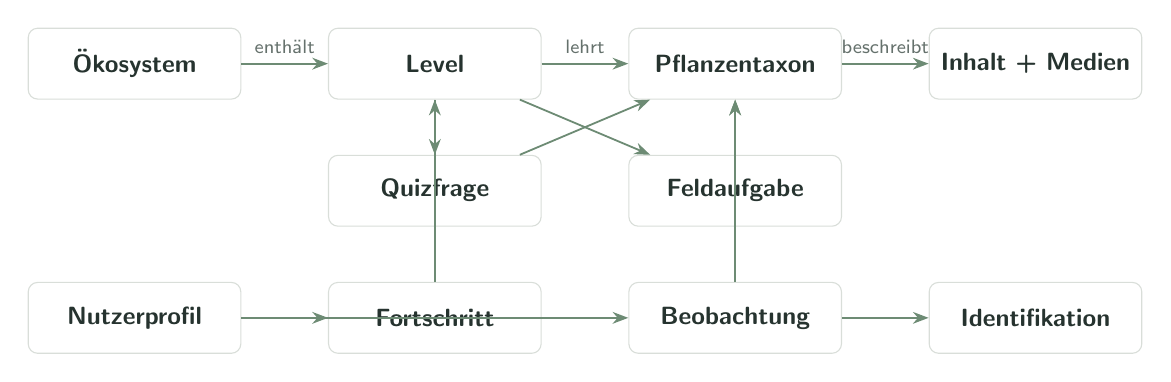
\begin{tikzpicture}[
  node distance=7mm and 11mm,
  entity/.style={draw=Line,fill=white,rounded corners=1.2mm,minimum width=27mm,minimum height=9mm,font=\small\bfseries,text=Ink},
  rel/.style={-{Stealth[length=2mm]},draw=Sage,line width=.65pt},
  note/.style={font=\scriptsize,text=Muted,align=center}]
  \node[entity] (eco) {Ökosystem};
  \node[entity,right=of eco] (level) {Level};
  \node[entity,right=of level] (plant) {Pflanzentaxon};
  \node[entity,right=of plant] (content) {Inhalt + Medien};
  \node[entity,below=of level] (quiz) {Quizfrage};
  \node[entity,below=of plant] (task) {Feldaufgabe};
  \node[entity,below=of task] (obs) {Beobachtung};
  \node[entity,left=of obs] (progress) {Fortschritt};
  \node[entity,left=of progress] (user) {Nutzerprofil};
  \node[entity,right=of obs] (ident) {Identifikation};
  \draw[rel] (eco) -- node[note,above]{enthält} (level);
  \draw[rel] (level) -- node[note,above]{lehrt} (plant);
  \draw[rel] (plant) -- node[note,above]{beschreibt} (content);
  \draw[rel] (level) -- (quiz);
  \draw[rel] (quiz) -- (plant);
  \draw[rel] (level) -- (task);
  \draw[rel] (task) -- (plant);
  \draw[rel] (user) -- (progress);
  \draw[rel] (progress) -- (level);
  \draw[rel] (user) -- (obs);
  \draw[rel] (obs) -- (plant);
  \draw[rel] (obs) -- (ident);
\end{tikzpicture}}
\end{center}

\begin{decisionbox}[title={\textbf{Taxonomische Stabilität}}]
Wissenschaftliche Namen können sich ändern. Beziehungen verwenden daher eine interne, unveränderliche Taxon-ID und -- soweit vorhanden -- externe Referenzen (z.\,B. GBIF/POWO/PlantNet). Namen und Synonyme sind versionierte Attribute, nicht Primärschlüssel. So bleiben Fortschritt und Herbarium bei taxonomischen Aktualisierungen erhalten.
\end{decisionbox}

% -----------------------------------------------------------------------------
\section{Ablaufbeschreibungen und Interaktionen}\label{sec:game-loop}

\subsection{Nutzungsablauf: Lernen bis Feldfund}

\begin{center}
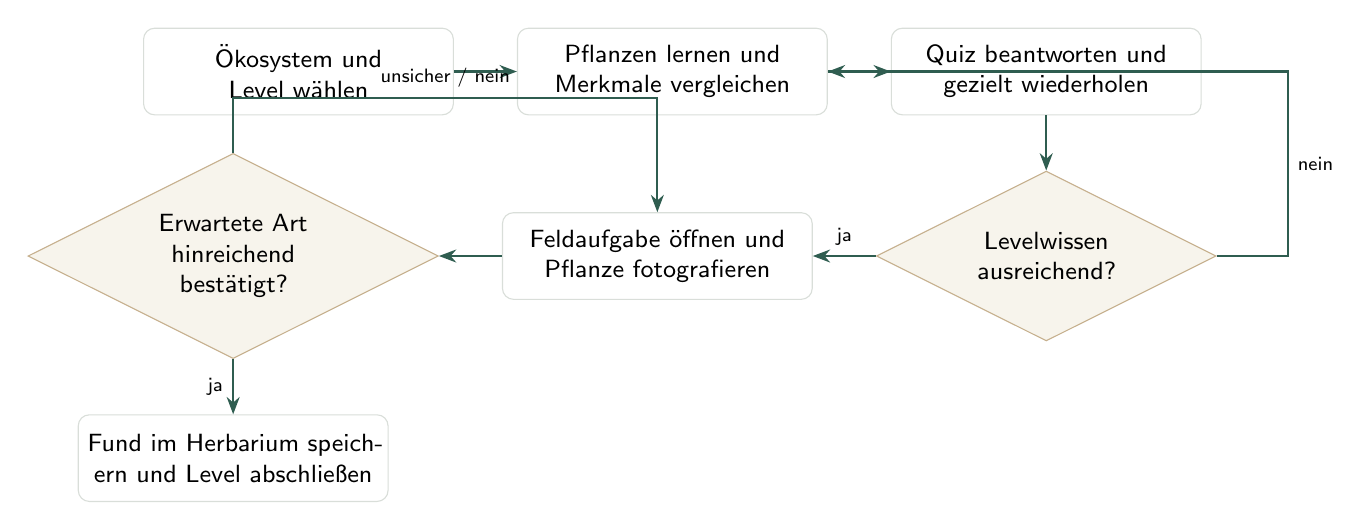
\begin{tikzpicture}[
  node distance=7mm and 8mm,
  flowstep/.style={draw=Line,fill=white,rounded corners=1.4mm,text width=37mm,minimum height=11mm,align=center,font=\small},
  decision/.style={diamond,draw=Sand!80!Bark,fill=Cream,aspect=2,text width=24mm,align=center,font=\small},
  arr/.style={-{Stealth[length=2.2mm]},draw=Forest,line width=.75pt}]
  \node[flowstep] (select) {Ökosystem und Level wählen};
  \node[flowstep,right=of select] (learn) {Pflanzen lernen und Merkmale vergleichen};
  \node[flowstep,right=of learn] (quiz) {Quiz beantworten und gezielt wiederholen};
  \node[decision,below=of quiz] (ready) {Levelwissen ausreichend?};
  \node[flowstep,left=of ready] (field) {Feldaufgabe öffnen und Pflanze fotografieren};
  \node[decision,left=of field] (match) {Erwartete Art hinreichend bestätigt?};
  \node[flowstep,below=of match] (herb) {Fund im Herbarium speichern und Level abschließen};
  \draw[arr] (select) -- (learn);
  \draw[arr] (learn) -- (quiz);
  \draw[arr] (quiz) -- (ready);
  \draw[arr] (ready) -- node[above,font=\scriptsize]{ja} (field);
  \draw[arr] (ready.east) -- ++(9mm,0) |- node[pos=.25,right,font=\scriptsize]{nein} (learn.east);
  \draw[arr] (field) -- (match);
  \draw[arr] (match) -- node[left,font=\scriptsize]{ja} (herb);
  \draw[arr] (match.north) -- ++(0,7mm) -| node[pos=.25,above,font=\scriptsize]{unsicher / nein} (field.north);
\end{tikzpicture}
\end{center}

\subsection{Spielschleife und Levelzustände}

Die Spielmechanik verbindet kurze Lernsitzungen mit einem realen Naturtransfer. Ein Level wird nicht durch reine Nutzungsdauer abgeschlossen, sondern durch eine konfigurierbare Kombination aus bearbeiteten Inhalten, Quizsicherheit und Feldnachweis. Fehler führen in eine gezielte Wiederholungsschleife; bereits erworbenes Wissen bleibt sichtbar.

\begin{center}
\resizebox{\textwidth}{!}{%
\begin{tikzpicture}[
  node distance=8mm and 10mm,
  phase/.style={draw=Line,fill=white,rounded corners=1.4mm,text width=31mm,minimum height=12mm,align=center,font=\small\bfseries},
  gate/.style={diamond,draw=Sand!80!Bark,fill=Cream,aspect=2.0,text width=21mm,align=center,font=\scriptsize\bfseries},
  arr/.style={-{Stealth[length=2.1mm]},draw=Forest,line width=.75pt},
  loop/.style={-{Stealth[length=2mm]},draw=Bark,dashed,line width=.65pt}]
  \node[phase,fill=Cream] (discover) {1 · Entdecken\\Ökosystem wählen};
  \node[phase,right=of discover] (learn) {2 · Lernen\\Arten + Merkmale};
  \node[phase,right=of learn] (practice) {3 · Üben\\gemischte Quizmodi};
  \node[gate,below=of practice] (mastery) {Schwelle erreicht?};
  \node[phase,left=of mastery] (field) {4 · Anwenden\\Feldaufgabe};
  \node[phase,left=of field] (identify) {5 · Prüfen\\PlantNet-Abgleich};
  \node[gate,below=of identify] (match) {Zielart bestätigt?};
  \node[phase,right=of match,fill=MustBg] (collect) {6 · Sammeln\\Herbarium + Erfolg};
  \node[phase,right=of collect] (repeat) {7 · Festigen\\Wiederholung später};
  \draw[arr] (discover) -- (learn);
  \draw[arr] (learn) -- (practice);
  \draw[arr] (practice) -- (mastery);
  \draw[arr] (mastery) -- node[above,font=\scriptsize]{ja} (field);
  \draw[arr] (field) -- (identify);
  \draw[arr] (identify) -- (match);
  \draw[arr] (match) -- node[above,font=\scriptsize]{ja} (collect);
  \draw[arr] (collect) -- (repeat);
  \draw[loop] (mastery.east) -- ++(9mm,0) |- node[pos=.24,right,font=\scriptsize]{nein: unsichere Arten} (learn.east);
  \draw[loop] (match.west) -- ++(-10mm,0) |- node[pos=.25,left,font=\scriptsize]{nein/unsicher: Tipps + neuer Versuch} (field.west);
  \draw[loop] (repeat.north) -- ++(0,8mm) -| node[pos=.35,above,font=\scriptsize]{nächstes Level oder Wiederholung} (discover.south);
\end{tikzpicture}}
\end{center}

\begin{tabularx}{\textwidth}{@{}p{31mm}X X@{}}
\toprule
\textbf{Zustand} & \textbf{Eintritt / gespeicherter Stand} & \textbf{Möglicher Übergang} \\
\midrule
Gesperrt & Voraussetzungen des Vorgängerlevels nicht erfüllt & Freigabe nach konfigurierbarer Abschlussregel \\
Aktiv & erste Lerneinheit gestartet; Fortschritt lokal ereignisbasiert & Lernen, Quiz, Pause, Gerätewechsel/Sync \\
Feldbereit & Lern- und Quizschwelle erreicht & Feldaufgabe starten oder Wissen weiter festigen \\
Nachweis ausstehend & Aufnahme lokal gespeichert oder Identifikationsauftrag läuft & Ergebnis, Retry, Offline-Warteschlange \\
Abgeschlossen & Abschlussregel serverseitig bestätigt & Herbariumseintrag, Erfolg, nächstes Level \\
Wiederholung fällig & Wiederholungsregel oder Unsicherheitsprofil greift & fokussiertes Quiz ohne Verlust des Abschlusses \\
\bottomrule
\end{tabularx}

Die Zustandswechsel beziehen sich insbesondere auf \R{FA020}--\R{FA029}, \R{FA030}--\R{FA040} und \R{FA041}--\R{FA045}. Schwellenwerte, Anzahl der Feldnachweise und Wiederholungsintervalle sind Inhaltskonfiguration, keine fest codierten App-Regeln.

\subsection{Technischer Ablauf: Fotoidentifikation}

\begin{center}
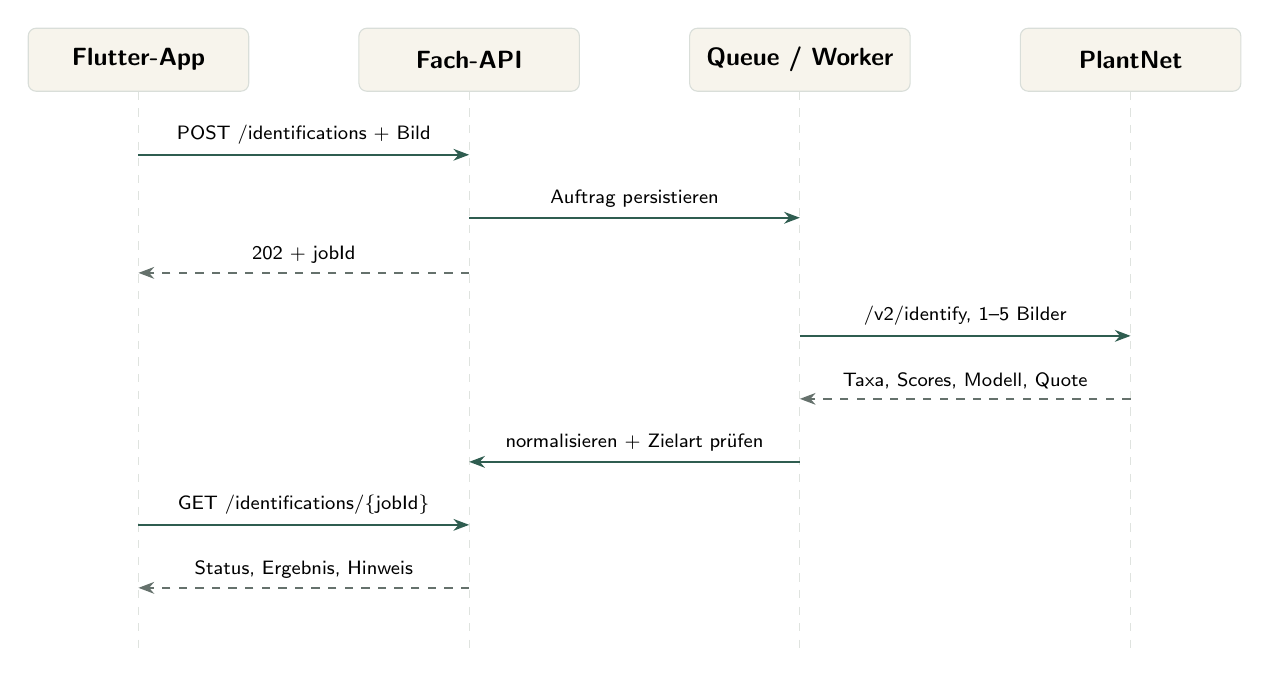
\begin{tikzpicture}[
  actor/.style={draw=Line,fill=Cream,rounded corners=1mm,minimum width=28mm,minimum height=8mm,font=\small\bfseries},
  life/.style={draw=Line!85,dashed},
  msg/.style={-{Stealth[length=2mm]},draw=Forest,line width=.65pt},
  ret/.style={-{Stealth[length=2mm]},draw=Muted,dashed,line width=.55pt},
  font=\scriptsize]
  \node[actor] (app) at (0,0) {Flutter-App};
  \node[actor] (api) at (4.2,0) {Fach-API};
  \node[actor] (queue) at (8.4,0) {Queue / Worker};
  \node[actor] (pn) at (12.6,0) {PlantNet};
  \foreach \n in {app,api,queue,pn}{\draw[life] (\n.south) -- ++(0,-7.1);}
  \draw[msg] ([yshift=-.8cm]app.south) -- node[above]{POST /identifications + Bild} ([yshift=-.8cm]api.south);
  \draw[msg] ([yshift=-1.6cm]api.south) -- node[above]{Auftrag persistieren} ([yshift=-1.6cm]queue.south);
  \draw[ret] ([yshift=-2.3cm]api.south) -- node[above]{202 + jobId} ([yshift=-2.3cm]app.south);
  \draw[msg] ([yshift=-3.1cm]queue.south) -- node[above]{/v2/identify, 1--5 Bilder} ([yshift=-3.1cm]pn.south);
  \draw[ret] ([yshift=-3.9cm]pn.south) -- node[above]{Taxa, Scores, Modell, Quote} ([yshift=-3.9cm]queue.south);
  \draw[msg] ([yshift=-4.7cm]queue.south) -- node[above]{normalisieren + Zielart prüfen} ([yshift=-4.7cm]api.south);
  \draw[msg] ([yshift=-5.5cm]app.south) -- node[above]{GET /identifications/\{jobId\}} ([yshift=-5.5cm]api.south);
  \draw[ret] ([yshift=-6.3cm]api.south) -- node[above]{Status, Ergebnis, Hinweis} ([yshift=-6.3cm]app.south);
\end{tikzpicture}
\end{center}

PlantNet liefert eine absteigend sortierte Trefferliste mit Scores von 0 bis 1, akzeptiert bis zu fünf JPG-/PNG-Bilder desselben Individuums und erlaubt Organangaben.\Src{2} Die eigene API muss die Antwort taxonomisch normalisieren und Unsicherheit fachlich darstellen. Die App darf den externen API-Key niemals erhalten.

\subsection{Technischer Ablauf: Offline-Synchronisation}

\begin{enumerate}[leftmargin=7mm,label=\textcolor{Forest}{\arabic*.}]
  \item Der Client lädt das aktuelle Manifest und vergleicht Versionen/Prüfsummen.
  \item Fehlende Inhaltsobjekte und Medien werden als Delta geladen und zunächst in einer Staging-Collection gespeichert.
  \item Erst nach erfolgreicher Validierung wird die neue Inhaltsversion atomar aktiviert.
  \item Lokale Lernereignisse werden in Batches mit stabilen Client-IDs übertragen; der Server quittiert bereits bekannte IDs idempotent.
  \item Persönliche Änderungen tragen Basisversionen. Bei konkurrierenden Notizen erhält die zuletzt editierende Person einen sichtbaren Konflikt statt stiller Überschreibung.
  \item Der Server antwortet mit autoritativen Fortschrittsständen, Löschmarken und dem nächsten Sync-Cursor.
\end{enumerate}

\subsection{Redaktioneller Ablauf}

\begin{center}
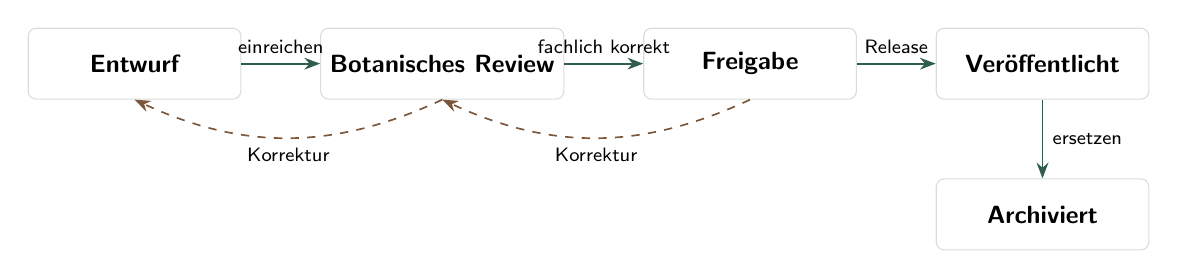
\begin{tikzpicture}[
  state/.style={draw=Line,fill=white,rounded corners=1mm,minimum width=27mm,minimum height=9mm,font=\small\bfseries},
  arr/.style={-{Stealth[length=2mm]},draw=Forest,line width=.7pt},
  back/.style={-{Stealth[length=2mm]},draw=Bark,dashed,line width=.6pt}]
  \node[state] (draft) {Entwurf};
  \node[state,right=of draft] (review) {Botanisches Review};
  \node[state,right=of review] (approve) {Freigabe};
  \node[state,right=of approve] (publish) {Veröffentlicht};
  \node[state,below=of publish] (archive) {Archiviert};
  \draw[arr] (draft) -- node[above,font=\scriptsize]{einreichen} (review);
  \draw[arr] (review) -- node[above,font=\scriptsize]{fachlich korrekt} (approve);
  \draw[arr] (approve) -- node[above,font=\scriptsize]{Release} (publish);
  \draw[arr] (publish) -- node[right,font=\scriptsize]{ersetzen} (archive);
  \draw[back] (review.south) to[bend left=25] node[below,font=\scriptsize]{Korrektur} (draft.south);
  \draw[back] (approve.south) to[bend left=25] node[below,font=\scriptsize]{Korrektur} (review.south);
\end{tikzpicture}
\end{center}

% -----------------------------------------------------------------------------
\section{Plattformarchitektur}\label{sec:architecture}

\subsection{Architekturprinzipien}

\begin{itemize}
  \item \textbf{App-zentrierte Entwicklung:} Standardfunktionen für Content, Medien, Rollen und Veröffentlichung werden aus einem etablierten Headless-CMS bezogen; Individualentwicklung konzentriert sich auf Lernen, Offline-Sync, Fortschritt, Herbarium und PlantNet.
  \item \textbf{Zentrale Identität:} Keycloak ist Vertrauensstelle für klassische Anmeldung, Google, Apple sowie institutionelles OIDC oder SAML. Das Fachbackend speichert nur die stabile Subject-ID und fachliche Profile.
  \item \textbf{Backend-for-Frontend:} Die Flutter-App greift nicht direkt auf Strapi-Admin- oder PlantNet-Endpunkte zu. Eine schlanke Fach-API stabilisiert mobile Verträge, Berechtigungen, Sync und Domänenregeln.
  \item \textbf{Offline first:} Der Client arbeitet lokal schnell; veröffentlichte Inhalte und endgültiger Abschlussstatus werden serverseitig autoritativ versioniert.
  \item \textbf{Asynchrone Medienverarbeitung:} Identifikation, Bildvarianten, Exporte und große Imports laufen über persistente Aufträge, damit externe Latenz keine App-Anfrage blockiert.
  \item \textbf{Offene Schnittstellen:} REST/OpenAPI, PostgreSQL, S3-kompatible Objektspeicherung, OIDC/SAML und standardisierte Exporte reduzieren Lock-in.
\end{itemize}

\subsection{Gesamtsystem}

\begin{center}
\resizebox{\textwidth}{!}{%
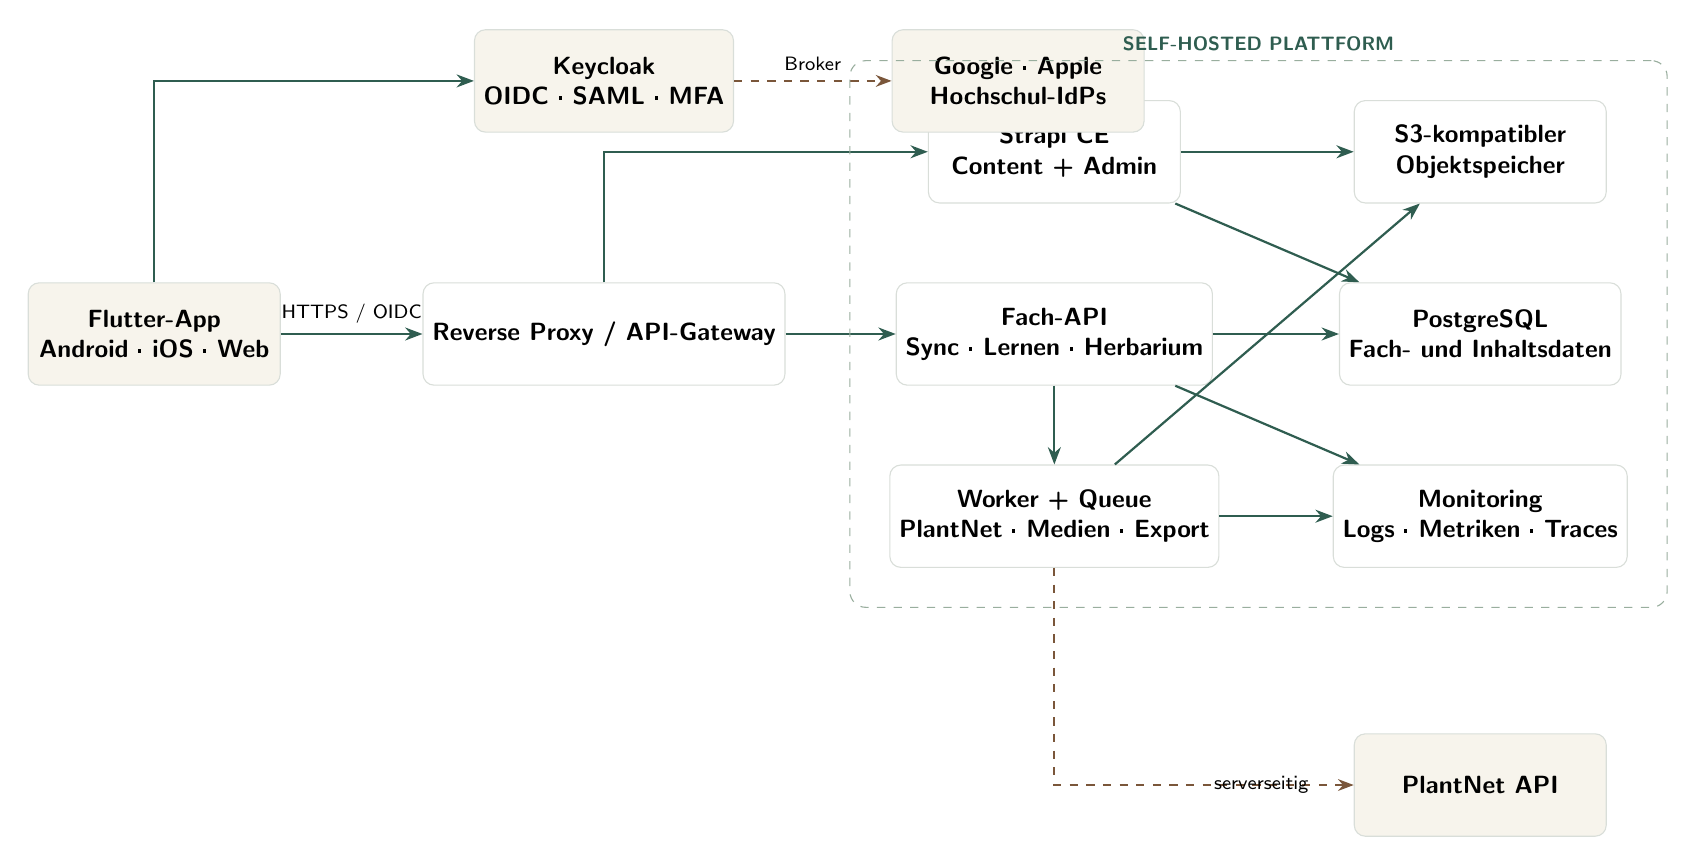
\begin{tikzpicture}[
  comp/.style={draw=Line,fill=white,rounded corners=1.4mm,minimum width=32mm,minimum height=13mm,align=center,font=\small\bfseries},
  group/.style={draw=Sage!70,dashed,rounded corners=2mm,inner sep=5mm},
  arr/.style={-{Stealth[length=2.2mm]},draw=Forest,line width=.8pt},
  ext/.style={-{Stealth[length=2mm]},draw=Bark,dashed,line width=.65pt}]
  \node[comp,fill=Cream] (app) {Flutter-App\\Android · iOS · Web};
  \node[comp,right=18mm of app] (gateway) {Reverse Proxy / API-Gateway};
  \node[comp,right=14mm of gateway] (api) {Fach-API\\Sync · Lernen · Herbarium};
  \node[comp,above=10mm of api] (cms) {Strapi CE\\Content + Admin};
  \node[comp,below=10mm of api] (worker) {Worker + Queue\\PlantNet · Medien · Export};
  \node[comp,right=16mm of api] (db) {PostgreSQL\\Fach- und Inhaltsdaten};
  \node[comp,above=10mm of db] (object) {S3-kompatibler\\Objektspeicher};
  \node[comp,below=10mm of db] (obs) {Monitoring\\Logs · Metriken · Traces};
  \node[comp,above=19mm of gateway,fill=Cream] (idp) {Keycloak\\OIDC · SAML · MFA};
  \node[comp,right=20mm of idp,fill=Cream] (social) {Google · Apple\\Hochschul-IdPs};
  \node[comp,below=21mm of obs,fill=Cream] (plantnet) {PlantNet API};

  \draw[arr] (app) -- node[above,font=\scriptsize]{HTTPS / OIDC} (gateway);
  \draw[arr] (gateway) -- (api);
  \draw[arr] (gateway) |- (cms);
  \draw[arr] (api) -- (db);
  \draw[arr] (cms) -- (db);
  \draw[arr] (api) -- (worker);
  \draw[arr] (worker) -- (object);
  \draw[arr] (cms) -- (object);
  \draw[arr] (api) -- (obs);
  \draw[arr] (worker) -- (obs);
  \draw[arr] (app) |- (idp);
  \draw[ext] (idp) -- node[above,font=\scriptsize]{Broker} (social);
  \draw[ext] (worker) |- node[pos=.75,right,font=\scriptsize]{serverseitig} (plantnet);
  \node[group,fit=(api)(cms)(worker)(db)(object)(obs),label={[font=\scriptsize\bfseries,text=Forest]above:SELF-HOSTED PLATTFORM}] {};
\end{tikzpicture}}
\end{center}

\subsection{Flutter-Architektur}

\begin{tabularx}{\textwidth}{@{}p{34mm}X X@{}}
\toprule
\textbf{Schicht} & \textbf{Verantwortung} & \textbf{Beispiele} \\
\midrule
Presentation & Screens, Zustände, Navigation, Accessibility, ViewModels/BLoCs & Levelansicht, Kamera, Herbarium, Syncstatus \\
Application & Orchestrierte Use Cases und Transaktionen & StartLevel, SubmitQuiz, QueueObservation, SyncContent \\
Domain & Reine Regeln, Entitäten und Ports & Levelabschluss, TaxonMatch, ProgressEvent, Repositories \\
Infrastructure & Adapter für Isar/Web-Store, HTTP, Kamera, GPS, Dateien und Telemetrie & IsarRepository, ApiClient, LocationAdapter \\
\bottomrule
\end{tabularx}

Features werden vertikal modularisiert (\Code{auth}, \Code{catalog}, \Code{learning}, \Code{quiz}, \Code{field}, \Code{herbarium}, \Code{sync}, \Code{profile}). Gemeinsame Domänenobjekte liegen in klar begrenzten Kernmodulen. Das Persistenzinterface darf weder Isar-Typen noch Web-APIs in die Domäne leaken.

\subsubsection{Komponentenstruktur innerhalb der App}\label{sec:app-components}

\begin{center}
\resizebox{\textwidth}{!}{%
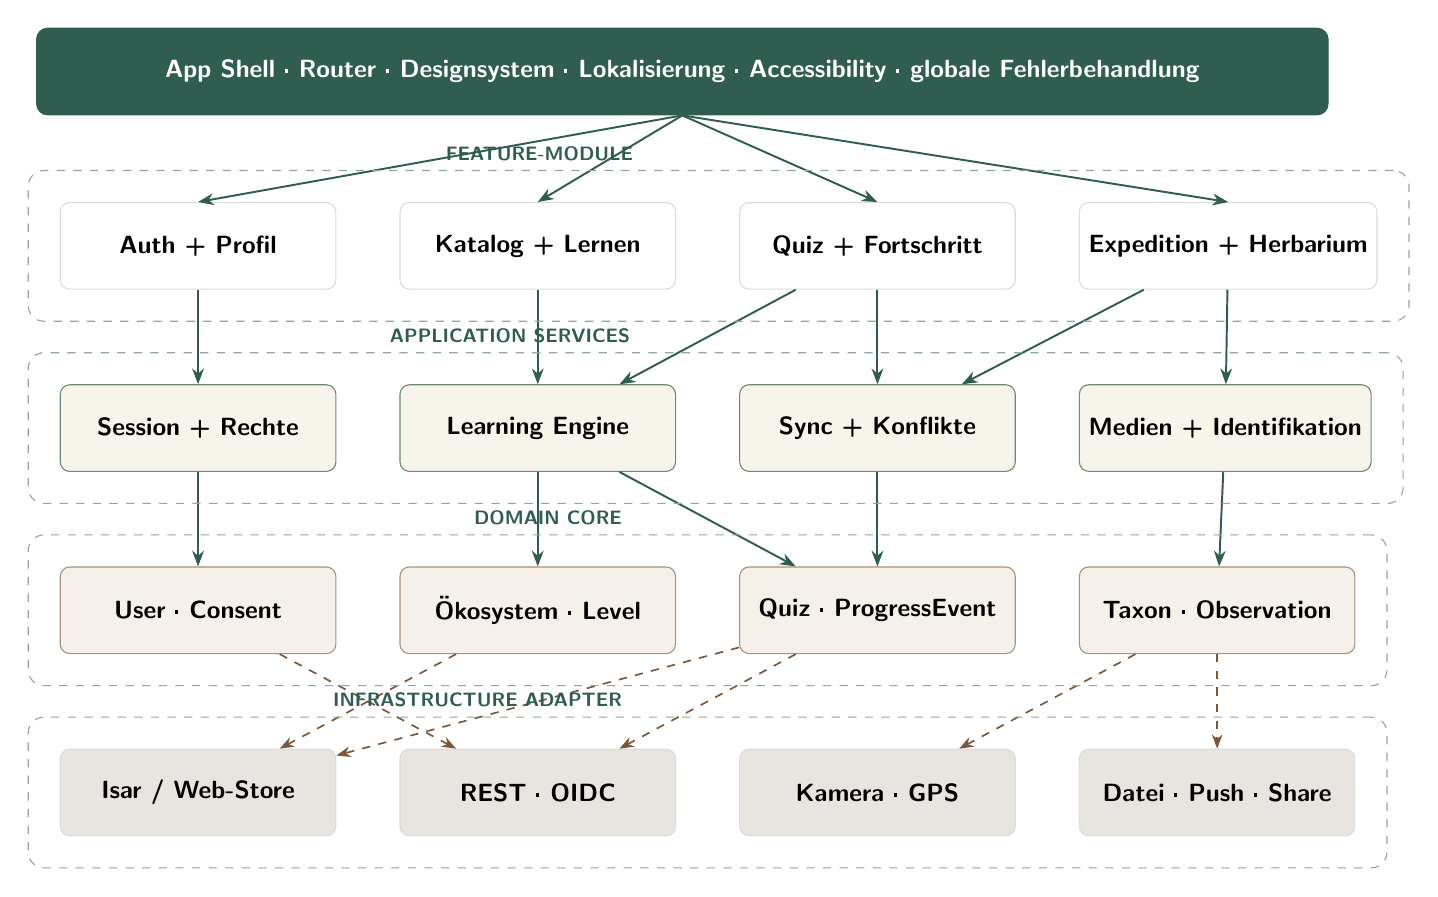
\begin{tikzpicture}[
  shell/.style={draw=Forest,fill=Forest,text=white,rounded corners=1.4mm,minimum height=11mm,align=center,font=\small\bfseries},
  feature/.style={draw=Line,fill=white,rounded corners=1.2mm,minimum width=35mm,minimum height=11mm,align=center,font=\small\bfseries},
  service/.style={draw=Sage,fill=Cream,rounded corners=1.2mm,minimum width=35mm,minimum height=11mm,align=center,font=\small\bfseries},
  domnode/.style={draw=Bark!65,fill=Beige!45,rounded corners=1.2mm,minimum width=35mm,minimum height=11mm,align=center,font=\small\bfseries},
  adapter/.style={draw=Line,fill=CouldBg,rounded corners=1.2mm,minimum width=35mm,minimum height=11mm,align=center,font=\small\bfseries},
  group/.style={draw=Sage!75,dashed,rounded corners=2mm,inner sep=4mm},
  dep/.style={-{Stealth[length=2mm]},draw=Forest,line width=.7pt},
  port/.style={-{Stealth[length=1.8mm]},draw=Bark,dashed,line width=.6pt}]
  \node[shell,minimum width=164mm] (shell) {App Shell · Router · Designsystem · Lokalisierung · Accessibility · globale Fehlerbehandlung};

  \node[feature,below=11mm of shell,xshift=-61.5mm] (auth) {Auth + Profil};
  \node[feature,right=8mm of auth] (catalog) {Katalog + Lernen};
  \node[feature,right=8mm of catalog] (quiz) {Quiz + Fortschritt};
  \node[feature,right=8mm of quiz] (field) {Expedition + Herbarium};

  \node[service,below=12mm of auth] (session) {Session + Rechte};
  \node[service,right=8mm of session] (engine) {Learning Engine};
  \node[service,right=8mm of engine] (sync) {Sync + Konflikte};
  \node[service,right=8mm of sync] (media) {Medien + Identifikation};

  \node[domnode,below=12mm of session] (identity) {User · Consent};
  \node[domnode,right=8mm of identity] (curriculum) {Ökosystem · Level};
  \node[domnode,right=8mm of curriculum] (progress) {Quiz · ProgressEvent};
  \node[domnode,right=8mm of progress] (observation) {Taxon · Observation};

  \node[adapter,below=12mm of identity] (store) {Isar / Web-Store};
  \node[adapter,right=8mm of store] (network) {REST · OIDC};
  \node[adapter,right=8mm of network] (device) {Kamera · GPS};
  \node[adapter,right=8mm of device] (platform) {Datei · Push · Share};

  \foreach \f in {auth,catalog,quiz,field}{\draw[dep] (shell.south) -- (\f.north);}
  \draw[dep] (auth) -- (session);
  \draw[dep] (catalog) -- (engine);
  \draw[dep] (quiz) -- (engine);
  \draw[dep] (quiz) -- (sync);
  \draw[dep] (field) -- (media);
  \draw[dep] (field) -- (sync);
  \draw[dep] (session) -- (identity);
  \draw[dep] (engine) -- (curriculum);
  \draw[dep] (engine) -- (progress);
  \draw[dep] (sync) -- (progress);
  \draw[dep] (media) -- (observation);
  \draw[port] (identity) -- (network);
  \draw[port] (curriculum) -- (store);
  \draw[port] (progress) -- (store);
  \draw[port] (progress) -- (network);
  \draw[port] (observation) -- (device);
  \draw[port] (observation) -- (platform);
  \node[group,fit=(auth)(field),label={[font=\scriptsize\bfseries,text=Forest]above left:FEATURE-MODULE}] {};
  \node[group,fit=(session)(media),label={[font=\scriptsize\bfseries,text=Forest]above left:APPLICATION SERVICES}] {};
  \node[group,fit=(identity)(observation),label={[font=\scriptsize\bfseries,text=Forest]above left:DOMAIN CORE}] {};
  \node[group,fit=(store)(platform),label={[font=\scriptsize\bfseries,text=Forest]above left:INFRASTRUCTURE ADAPTER}] {};
\end{tikzpicture}}
\end{center}

\textbf{Abhängigkeitsregeln:}
\begin{itemize}
  \item Feature-Module kommunizieren nicht über fremde Widgets oder Datenbanktabellen, sondern über explizite Use Cases, Events und schmale öffentliche Verträge.
  \item Der Domain Core kennt Flutter, Isar, HTTP, Kamera, GPS und PlantNet nicht. Infrastructure Adapter implementieren die vom Domain-/Application-Layer definierten Ports.
  \item \Code{sync} ist Querschnittskomponente für Content-Releases, Lernereignisse und private Herbariumdaten; sie entscheidet nicht über fachliche Levelregeln.
  \item \Code{field} erzeugt eine lokale Beobachtung und einen Identifikationsauftrag. Erst ein Domain-Use-Case bewertet das normalisierte Ergebnis gegen die erwartete Zielart.
  \item Plattformunterschiede zwischen Android, iOS und Web enden hinter Adaptern; dieselben Widget-, Use-Case- und Domain-Tests laufen auf allen Zielplattformen.
\end{itemize}

\begin{decisionbox}[title={\textbf{Konkreter Modulzuschnitt für das MVP}}]
Pro Feature wird ein Package-Verzeichnis mit \Code{presentation}, \Code{application}, \Code{domain} und \Code{infrastructure} angelegt. Kleine Features dürfen Schichten physisch zusammenfassen, solange die Abhängigkeitsrichtung eingehalten bleibt. Wiederverwendbare UI-Bausteine liegen in \Code{design\_system}; fachliche Sammelklassen in einem unkontrollierten \Code{shared}-Ordner sind zu vermeiden. Damit bleiben Quiztypen, Speicheradapter und Identifikationslogik unabhängig austausch- und testbar (\R{NFA002}, \R{NFA021}).
\end{decisionbox}

\subsection{Backend-Komponenten}

\begin{tabularx}{\textwidth}{@{}p{39mm}X p{44mm}@{}}
\toprule
\textbf{Komponente} & \textbf{Aufgabe} & \textbf{Technologieentscheidung} \\
\midrule
Headless CMS / Administration & Inhalte, Medienmetadaten, Beziehungen, Draft/Publish, Rollen, Redaktion & Strapi Community Edition, TypeScript \\
Fach-API & stabile App-Endpunkte, Sync, Fortschritt, Feldaufgaben, Herbarium, Datenschutz & Strapi-Erweiterung oder separater schlanker TypeScript-Service; Entscheidung nach Spike \\
Identity Provider & Login, Provider-Broker, MFA, Institutionen, Token & Keycloak \\
Relationale Datenbank & konsistente Inhalts-, Fach- und Auditdaten & PostgreSQL \\
Objektspeicher & Originale, Varianten, private Nutzerfotos, Exporte & S3-kompatibel, EU/self-hosted \\
Queue / Worker & Identifikation, Medien, Import, Export, Löschläufe & Redis-kompatible Queue oder PostgreSQL-Queue; persistent \\
Observability & Metriken, Logs, Traces, Alarmierung & OpenTelemetry-kompatibler OSS-Stack \\
\bottomrule
\end{tabularx}

\subsection{Deployment-Topologie}

Für den MVP genügt ein hochverfügbar vorbereiteter, aber bewusst einfacher Betrieb: zwei API-/CMS-Instanzen hinter Reverse Proxy, mindestens ein separater Worker, verwaltetes oder repliziertes PostgreSQL, redundanter Objektspeicher/Backup und getrenntes Staging. Kubernetes ist nicht zwingend; Docker/Podman-Compose oder Nomad kann bei der erwarteten Last kostengünstiger und wartbarer sein. Die Deploymentform muss automatisiert und portabel sein, nicht maximal komplex.

% -----------------------------------------------------------------------------
\section{Backend-Evaluation und Entscheidung}\label{sec:backend-decision}

\subsection{Entscheidungskriterien}

Das Backend soll möglichst viel Standardfunktion bereitstellen, ohne Open Source, Self-Hosting und Erweiterbarkeit zu gefährden. Bewertet werden Lizenz, visuelle Inhaltsmodellierung, Redaktion, REST/GraphQL, Medien, Mehrsprachigkeit und Rollen. Hinzu kommen Veröffentlichung, PostgreSQL, Auth-Integration, Betrieb und Lock-in.

\begin{table}[htbp]
\centering
\small
\begin{tabularx}{\textwidth}{@{}p{28mm}*{5}{>{\centering\arraybackslash}X}@{}}
\toprule
\textbf{Kriterium} & \textbf{Strapi CE} & \textbf{Payload} & \textbf{Directus} & \textbf{Supabase} & \textbf{Appwrite} \\
\midrule
Open-Source-Kern & ++ (MIT) & ++ (MIT) & $\circ$ Lizenz-/Tierprüfung & ++ & ++ \\
Redaktion / CMS & ++ & + & ++ & -- & -- \\
Visuelles Datenmodell & ++ & -- (Code-first) & ++ & $\circ$ DB-first & $\circ$ \\
REST / GraphQL & ++ & ++ & ++ & ++ & + \\
Medien / i18n / Publish & ++ & ++ & ++ & $\circ$ Eigenbau & $\circ$ Eigenbau \\
App-Fachlogik & + erweiterbar & ++ erweiterbar & + Flows/Extensions & + Functions/RLS & + Functions \\
Institutionelles SSO & über Keycloak / Adapter & über Keycloak / Adapter & je Tier prüfen & OIDC/Keycloak möglich & OIDC möglich \\
Betriebsaufwand & mittel & mittel & mittel & hoch (viele Dienste) & hoch (viele Dienste) \\
MVP-Fit & \textbf{sehr hoch} & hoch & hoch mit Lizenzrisiko & mittel & mittel \\
\bottomrule
\end{tabularx}
\end{table}

Strapi generiert für Content Types REST/GraphQL-APIs, bietet visuellen Content-Type-Builder, Media Library, Internationalisierung, Draft/Publish, Rollen und ein erweiterbares Adminsystem.\Src{4} Die selbst gehostete Open-Source-Ausgabe wird als MIT-lizenziert und ohne Nutzungsgrenzen ausgewiesen.\Src{5} Payload ist technisch ebenfalls sehr attraktiv und vollständig codezentriert: Admin, Datenbankmigrationen, REST/GraphQL, Auth, Access Control und Uploads entstehen aus TypeScript-Konfiguration.\Src{6} Für ein Projekt, in dem nichttechnische Arbeitsgruppen das Inhaltsmodell und große Mengen Lehrinhalt pflegen, ist Strapis visuelle Modellierung im MVP jedoch vorteilhafter.

Directus wäre redaktionell besonders stark, seine aktuelle Core-/Tier-Lizenz und SSO-Verfügbarkeit sind jedoch organisationsabhängig und müssen gegen die Forderung „vollständig Open Source“ bewertet werden; die offizielle Preisseite nennt Organisationsgrenzen und SSO erst in höheren Tiers.\Src{7} Supabase ist ein portabler Open-Source-PostgreSQL-Stack mit Auth, Data API und Storage, bietet aber keine fachlich passende Lerninhaltsredaktion; zu viel Admin-UI und Workflow müsste selbst gebaut werden.\Src{8}

\begin{decisionbox}[title={\textbf{ADR-BE-001 -- Empfohlenes Backend}}]
\textbf{Entscheidung: Strapi Community Edition + PostgreSQL + Keycloak + S3-kompatibler Objektspeicher.}

Strapi übernimmt Inhaltsmodelle, Medien, Redaktionsoberfläche, Internationalisierung und Veröffentlichungsbasis. Keycloak übernimmt sämtliche App-Identitäten und externes SSO; es unterstützt standardisiert OIDC, OAuth 2.0, SAML, Social Login, Identity Brokering sowie Benutzer-/Sitzungsverwaltung.\Src{9} Die projektspezifische Fach-API kapselt Fortschritt, Offline-Sync, Herbarium, PlantNet und Datenschutzprozesse. Dadurch bleibt der Implementierungsfokus auf der Flutter-App, während fachliche Regeln nicht in generische CMS-Endpunkte auslaufen.
\end{decisionbox}

\subsection{Warum nicht „nur Strapi“?}

Direkte generische CMS-CRUD-Aufrufe aus der App wären kurzfristig schnell, koppeln aber Client, Schema, Berechtigungen und Synchronisation zu eng. Eine dünne Fach-API ist notwendig für idempotente Ereignisse, atomare Inhaltsreleases, serverseitigen Levelabschluss, PlantNet-Keyschutz, Quotensteuerung, Standortminimierung und stabile mobile Verträge. Sie kann zunächst als Strapi-Plugin/Custom Routes umgesetzt und bei Wachstum in einen separaten Dienst extrahiert werden.

\subsection{Isar-Entscheidung und Web-Risiko}

Isar bleibt für Android/iOS gesetzt. Projektstatus und Web-Support waren zuletzt Gegenstand von Maintainer- und Community-Diskussionen; dies ist für ein Web-Ziel ein relevantes Liefer- und Governance-Risiko.\Src{10} Deshalb ist die lokale Datenbank eine Infrastrukturentscheidung hinter Repository-Ports. Bis Ende August 2026 muss ein Spike Kamera, große IDs, Migration, verschlüsselte/private Daten, Web-Storage-Limits und Offline-Sync im Zielbrowser nachweisen. Falls kein stabiler Isar-Webpfad verfügbar ist, verwendet Web einen IndexedDB-/Drift-WASM-Adapter bei identischem Domänenvertrag.

% -----------------------------------------------------------------------------
\section{API-Übersicht}\label{sec:api}

\subsection{Konventionen}

\begin{itemize}
  \item Basis: \Code{/api/v1}; JSON in UTF-8; Uploads per Multipart oder kurzlebiger signierter Upload-URL.
  \item Authentifizierung: OIDC Access Token; Autorisierung immer serverseitig; Scopes/Rollen werden auf Fachrechte abgebildet.
  \item Idempotenz: Schreibende Offline-Aufrufe tragen \Code{Idempotency-Key} bzw. stabile Client-ID.
  \item Paginierung: Cursor statt Offset bei veränderlichen Listen; \Code{ETag}/\Code{If-None-Match} für Inhaltsabfragen.
  \item Fehler: RFC-7807-artiges Problem-JSON mit stabilem Code, nutzergeeigneter Nachricht, Trace-ID und Feldfehlern.
  \item Versionierung: Hauptversion im Pfad; Inhaltsversion separat im Manifest; Deprecation-Header bei Ablösung.
\end{itemize}

\subsection{App- und Synchronisationsendpunkte}

\small
\begin{longtable}{@{}p{14mm}p{54mm}p{92mm}@{}}
\toprule
\textbf{Methode} & \textbf{Name / Pfad} & \textbf{Beschreibung} \\
\midrule
\endhead
GET & \Code{/me} & Fachprofil, Organisation, Locale, Rollen und Einwilligungsstatus des angemeldeten Kontos. \\
PATCH & \Code{/me} & Änderbare Profilfelder aktualisieren; keine Identitäts-/Passwortverwaltung. \\
GET & \Code{/content/manifest} & Aktuelle Inhaltsversion, Pakete, Prüfsummen, Größen, Mindest-App-Version und zurückgezogene Releases. \\
GET & \Code{/content/changes?since=} & Delta von Entitäten und Löschmarken ab Sync-Cursor. \\
GET & \Code{/ecosystems} & Veröffentlichte Ökosysteme, Region, Reihenfolge und Paketstatus. \\
GET & \Code{/ecosystems/\{id\}} & Ökosystemdetail mit Levelreferenzen und lokalisierten Metadaten. \\
GET & \Code{/levels/\{id\}} & Levelstruktur, Voraussetzungen, Lernblöcke, Quizmix und Abschlussregeln. \\
GET & \Code{/plants/\{id\}} & Kuratierter Steckbrief, Synonyme, Medienvarianten, Warnungen und Quellen. \\
GET & \Code{/quiz-items?levelId=} & Freigegebene Fragen bzw. signiertes Offline-Paket für ein Level. \\
POST & \Code{/learning-events:batch} & Idempotenter Batch lokaler Lern-/Quiz-/Fortschrittsereignisse. \\
GET & \Code{/progress} & Autoritativer Gesamtstand; optional seit Cursor oder je Level. \\
POST & \Code{/level-attempts} & Start/Resume eines Leveldurchlaufs, Rückgabe der Attempt-ID. \\
POST & \Code{/level-attempts/\{id\}:complete} & Servervalidierter Abschlussversuch mit erfüllten Nachweisen. \\
GET & \Code{/achievements} & Erreichte und nächste Erfolge, ohne geheime Kriterien offenzulegen. \\
POST & \Code{/sync} & Optionaler kombinierter Sync für kleine Batches: Events senden, Änderungen und Cursor empfangen. \\
\bottomrule
\end{longtable}

\subsection{Feld-, Identifikations- und Herbariumendpunkte}

\begin{longtable}{@{}p{14mm}p{54mm}p{92mm}@{}}
\toprule
\textbf{Methode} & \textbf{Name / Pfad} & \textbf{Beschreibung} \\
\midrule
\endhead
POST & \Code{/media/uploads} & Privaten Upload initialisieren oder kleine Datei annehmen; Typ/Größe/Hash validieren. \\
POST & \Code{/identifications} & Identifikationsauftrag mit Medien-IDs, Organen, Zielart, Region und Client-ID erstellen; liefert 202 + Job-ID. \\
GET & \Code{/identifications/\{jobId\}} & Status, normalisierte Kandidaten, Scores, Modell-/Quoteninfo und Zielabgleich. \\
POST & \Code{/identifications/\{jobId\}:retry} & Kontrollierter Retry nach neuem Bild oder vorübergehendem Providerfehler. \\
GET & \Code{/observations} & Eigene Herbariumliste mit Cursor, Suche und Filtern. \\
POST & \Code{/observations} & Eigenen Fund idempotent anlegen; genaue Geodaten als getrennt geschütztes Feld. \\
GET & \Code{/observations/\{id\}} & Eigenes Detail einschließlich Medien, Notiz und Identifikationshistorie. \\
PATCH & \Code{/observations/\{id\}} & Notiz, Datum und Standortfreigabe versionsgesichert ändern. \\
DELETE & \Code{/observations/\{id\}} & Löschmarke erzeugen, Medienlöschung asynchron ausführen. \\
POST & \Code{/observations/\{id\}:export} & Datenschutzgerechten Einzelfundexport erzeugen, GPS standardmäßig vergröbern. \\
\bottomrule
\end{longtable}

\subsection{Administration, Datenschutz und Forschung}

\begin{longtable}{@{}p{14mm}p{54mm}p{92mm}@{}}
\toprule
\textbf{Methode} & \textbf{Name / Pfad} & \textbf{Beschreibung} \\
\midrule
\endhead
POST & \Code{/admin/content-releases} & Validierten Inhaltsrelease/Manifest aus freigegebenen CMS-Daten erzeugen. \\
POST & \Code{/admin/imports} & Validierten Dry-run bzw. Importauftrag für Pflanzen/Quiz/Übersetzungen starten. \\
GET & \Code{/admin/dashboard} & Aggregierte Nutzungs- und Qualitätskennzahlen mit Zeitraum/Scope. \\
GET & \Code{/admin/users} & Berechtigte Nutzersuche mit Status und Organisation; keine Passwörter. \\
POST & \Code{/admin/users/\{id\}:suspend} & Konto sperren und Sitzungswiderruf anstoßen. \\
POST & \Code{/privacy/exports} & Gesamtdatenkopie der betroffenen Person anfordern. \\
POST & \Code{/privacy/deletions} & Kontolöschung anfordern, Status und etwaige Aufbewahrungsgründe liefern. \\
GET & \Code{/research/exports/\{id\}} & Nur für genehmigte Projekte: pseudonymisierten Export nach Freigabe laden. \\
\bottomrule
\end{longtable}
\normalsize

\subsection{PlantNet-Adapter}

Der Worker ruft für eine einzelne Pflanze \Code{POST /v2/identify/\{project\}} auf. PlantNet dokumentiert bis zu fünf Bilder desselben Individuums, Organangaben und Scores; Quoten werden täglich pro Request-Kategorie verwaltet und über Header bzw. Quotenendpunkte sichtbar.\Src{2}\Src{3} Das Backend hält mindestens folgende Adapterdaten fest: externe Request-ID, Referenzial/Projekt, Sprache, Anzahl/Bildorgane, Top-K-Kandidaten, Scores, wissenschaftliche Namen und externe IDs, Modellversion, Zeit, Quotenrest und Fehlerklasse. Rohbilder werden nicht länger als für Auftrag, Herbarium und Einwilligung erforderlich beim Dienst bzw. lokal gehalten.

% -----------------------------------------------------------------------------
\section{Last-, Wachstums- und Kapazitätsmodell}\label{sec:load}

\subsection{Annahmen der S-Kurve}

Die Nutzerangabe „anfangs 2 neue Nutzer:innen pro Tag, nach drei Monaten 2.000 pro Tag, am Ende nach sechs Monaten wieder 2 pro Tag“ beschreibt eine glockenförmige tägliche Akquisitionsrate; deren Integral ist die kumulative S-Kurve. Für eine transparente Planung wird für $0 \leq t \leq 180$ Tage verwendet:

\[
r(t)=2+1998\,\sin^2\!\left(\frac{\pi t}{180}\right)
\]

Damit gelten $r(0)=2$, $r(90)=2000$ und $r(180)=2$. Die kumulierten Registrierungen sind:

\[
U(t)=1001t-\frac{89910}{\pi}\sin\!\left(\frac{\pi t}{90}\right)
\]

Nach 180 Tagen ergibt das Modell rund \textbf{180.180 Konten}. Es ist ein Kapazitätsszenario, keine Marktprognose. Kampagnen, Semesterbeginn und Schulveranstaltungen können deutlich spitzere Last erzeugen.

\begin{center}
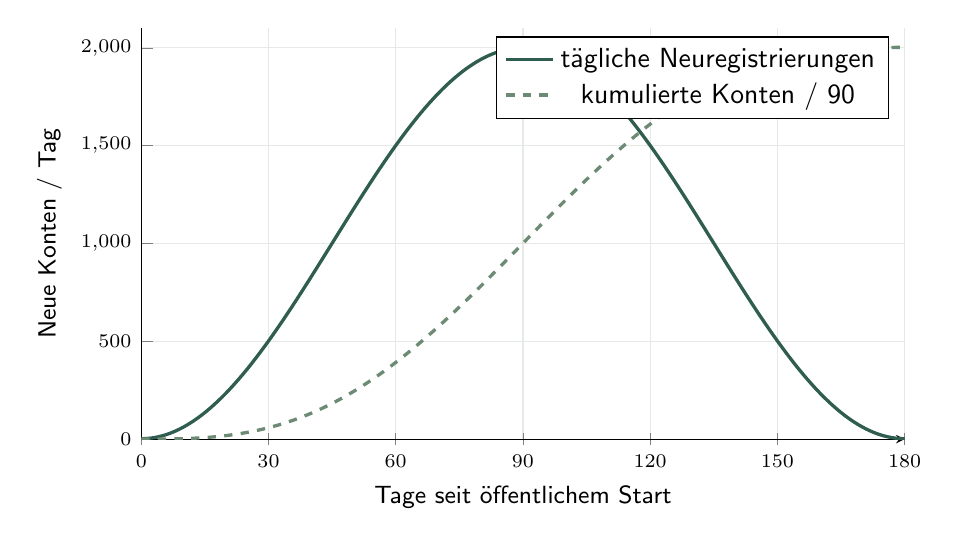
\begin{tikzpicture}
\begin{axis}[
  width=.93\textwidth,height=68mm,
  axis y line*=left,axis x line=bottom,
  xmin=0,xmax=180,ymin=0,ymax=2100,
  xlabel={Tage seit öffentlichem Start},ylabel={Neue Konten / Tag},
  xtick={0,30,60,90,120,150,180},
  ytick={0,500,1000,1500,2000},
  grid=major,grid style={Line!65},
  tick label style={font=\scriptsize},label style={font=\small},
  every axis plot/.append style={line width=1.2pt}]
  \addplot[Forest,domain=0:180,samples=181] {2+1998*(sin(deg(pi*x/180)))^2};
  \addplot[Sage,dashed,domain=0:180,samples=181] {(1001*x-(89910/pi)*sin(deg(pi*x/90)))/90};
  \legend{tägliche Neuregistrierungen,kumulierte Konten / 90}
\end{axis}
\end{tikzpicture}
\end{center}

\begin{table}[htbp]
\centering
\begin{tabular}{rrrr}
\toprule
\textbf{Tag} & \textbf{Neue/Tag} & \textbf{Kumuliert ca.} & \textbf{Planungsphase} \\
\midrule
0 & 2 & 0 & kontrollierter Start \\
30 & 502 & 5.245 & frühes Wachstum \\
60 & 1.501 & 35.275 & Beschleunigung \\
90 & 2.000 & 90.090 & Spitzenakquise \\
120 & 1.501 & 144.905 & Abflachung \\
150 & 502 & 174.935 & späte Adoption \\
180 & 2 & 180.180 & Plateau \\
\bottomrule
\end{tabular}
\end{table}

\subsection{Nutzungs- und Lastannahmen}

Für Dimensionierung, nicht als Produktziel, gelten am Wachstumsmaximum:

\begin{itemize}
  \item 15\,\% tägliche aktive Nutzer:innen (DAU) aus bis zu 180.000 Konten: ca. 27.000 DAU.
  \item 25 App-API-Aufrufe pro DAU/Tag nach Cache: ca. 675.000 Requests/Tag.
  \item 20\,\% der Tageslast in der stärksten Stunde entsprechen ca. 37,5 Requests/s im Mittel. Die Zielauslegung beträgt \textbf{100 RPS} plus Burstschutz.
  \item Im Mittel entstehen 0,2 Identifikationen pro DAU und damit ca. 5.400 PlantNet-Aufträge pro Tag. Exkursionstage werden mit Faktor 3 als Burst geplant (ca. 16.000/Tag).
  \item 3,0 MB optimiertes privates Foto je abgeschlossenem Fund: 16 GB neue Medien/Tag im Mittel, bis 48 GB an Exkursionstagen; Originalpolitik beeinflusst dies stark.
  \item 1,5 MB Offline-Inhaltsdaten plus 120 MB Medien pro vollständig geladenem MVP-Paket als Startbudget; tatsächliche Größe wird in der Content-Pipeline gemessen.
\end{itemize}

Das kostenlose PlantNet-Angebot erlaubt 500 Identifikationen pro Tag. Für Bildungs-/Wissenschaftsorganisationen nennt PlantNet ein kostenfreies Non-Profit-Modell mit mehr als 500 Identifikationen oder Burst-Nutzung auf Anfrage und verpflichtender „powered by Pl@ntNet“-Attribution. Der Pro-Tarif startet laut offizieller Preisseite mit Mindestabrechnung und volumenabhängigen Kosten.\Src{11} Vor Feldpilot muss daher ein Non-Profit-Vertrag oder ein belastbares kommerzielles Kontingent vorliegen; die freie Standardquote reicht für das Szenario nicht.

\subsection{Kapazitätsstufen}

\begin{tabularx}{\textwidth}{@{}p{25mm}p{33mm}X X@{}}
\toprule
\textbf{Stufe} & \textbf{Konten / Last} & \textbf{Technische Auslegung} & \textbf{Auslöser zum Ausbau} \\
\midrule
Pilot & bis 2.000, <10 RPS & 1--2 Appinstanzen, 1 Worker, PostgreSQL, S3, tägliche Backups & p95, Queue oder DB >60\,\% dauerhaft \\
Wachstum & bis 50.000, 10--50 RPS & 2+ API/CMS, 2 Worker, Redis/Queue, CDN, DB-Tuning/Read Cache & 70\,\% CPU/IO, PlantNet >70\,\% Quote \\
Zielhalbjahr & bis 200.000, 50--100 RPS & horizontale API/Worker, HA-DB, Lifecycle Storage, WAF/Rate Limit, Restore-Automation & Lasttest 2x Zielprofil vor Kampagne \\
International & >200.000 oder Regionen & regionale Medien/CDN, Partitionierung, getrennte Contentpakete, ggf. Service-Extraktion & gemessener Engpass, nicht Vorab-Komplexität \\
\bottomrule
\end{tabularx}

\subsection{Speicher- und Kostenhebel}

Der größte variable Kostenblock ist nicht JSON/API, sondern Nutzerfoto + Identifikationsvolumen. Bei 5.400 Fotos/Tag und 3 MB entstehen rund 5,9 TB/Jahr vor Replikation. Deshalb sind clientseitige Kompression, getrennte Thumbnail-/Originalpolitik, Lifecycle-Regeln, Löschung bei Kontolöschung und ein klarer Zweck für Originale zwingend. PlantNet-Kosten werden über Quotenmetrik, tägliche Warnschwellen und Warteschlange kontrolliert.

% -----------------------------------------------------------------------------
\section{Entwicklungs- und Einführungsplan bis April 2027}

\subsection{Rahmen}

Planungsbeginn ist der 20. Juli 2026; als konkreter Zieltermin wird \textbf{15. April 2027} angenommen. Die Planung umfasst etwa 39 Kalenderwochen. Alle MVP-Kernfunktionen sind enthalten, die botanische Inhaltsproduktion läuft parallel zur Softwareentwicklung. Förderbescheide dürfen wegen ihrer Vorlaufzeit nicht auf dem kritischen Pfad des April-Go-lives liegen.

\begin{longtable}{@{}p{23mm}p{36mm}p{99mm}@{}}
\toprule
\textbf{Zeitraum} & \textbf{Phase / Gate} & \textbf{Ergebnisse} \\
\midrule
\endhead
20.07.--14.08.2026 & P0 · Inception & Freigabe Scope/Artenzählung, Forschungsziele, Personas, Datenschutz-Screening, Lizenzstrategie, Contentinventar, Projektgovernance. \\
17.08.--11.09.2026 & P1 · Architektur-Spikes & Strapi-/Keycloak-Prototyp, Isar-Web-Spike, Offline-Sync-Prototyp, PlantNet-Vertrag/Quote, OpenAPI-Grundvertrag, CI-Basis. Gate A: Architekturfreigabe. \\
14.09.--30.10.2026 & P2 · Fundament & Flutter-Shell, Navigation/Designsystem, Auth inkl. Google/Apple/Test-IdP, Contentmodelle, Medienpipeline, API v1, Staging, Backup/Monitoring. \\
02.11.--18.12.2026 & P3 · Lernkern & Ökosysteme, Level, Steckbriefe, drei Quizmodi, Fortschritt, Downloads, Offline-Pakete, Admin-Builder, Draft/Review/Publish. Gate B: interner Alpha-Durchlauf. \\
04.01.--12.02.2027 & P4 · Feld und Sammlung & Kamera, Standortoption, Uploadqueue, PlantNet-Worker, Zielabgleich, Unsicherheits-UX, Herbarium, Sync zwischen Geräten, Datenschutzexport/-löschung. \\
15.02.--12.03.2027 & P5 · Integration und Inhalt & Nutzungsdashboard, Rechte-/Organisationsprüfung, 75 Arten vollständig, Levelkonfiguration, Übersetzungs- und Lizenzreview, Accessibility, Contract-/Lasttests. Gate C: Feature Complete. \\
15.03.--26.03.2027 & P6 · Feldpilot & Pilot mit Lehrenden/Lernenden im Botanischen Garten bzw. heimischen Ökosystem, Usability-/Lernfeedback, Fehlerbehebung, DSFA/Ethik/Store-Unterlagen. \\
29.03.--09.04.2027 & P7 · Release Candidate & Penetrationstest, Restore-/Rollbacktest, App-Store-Einreichung, Produktionsmigration, Support-/Incident-Übung, Go-live-Entscheidung. \\
15.04.2027 & M1 · Go-live & gestufte Freischaltung, enges Monitoring, Kommunikations- und Supportplan, tägliches Lagebild in der ersten Woche. \\
16.04.--30.04.2027 & P8 · Stabilisierung & Hotfixfenster, Quoten-/Kostenreview, Datenqualitätsprüfung, Retrospektive und Roadmap 1.1. \\
\bottomrule
\end{longtable}

\subsection{Meilensteine und Eintrittskriterien}

\begin{tabularx}{\textwidth}{@{}p{23mm}p{32mm}X@{}}
\toprule
\textbf{Gate} & \textbf{Termin} & \textbf{Mindestkriterien} \\
\midrule
A · Architektur & 11.09.2026 & Backend-/Lizenzentscheid, Isar-Web-Fallback, Auth-Prototyp, PlantNet-Kontingentweg, Datenschutzdatenfluss. \\
B · Alpha & 18.12.2026 & Ein Level Ende-zu-Ende offline spielbar, CMS-Publikation ohne App-Release, CI/Staging grün. \\
C · Feature Complete & 12.03.2027 & Alle MUSS-Funktionen implementiert, 75 Arten reviewt, keine offenen Blocker, Migrationen stabil. \\
D · Go-live & 09.04.2027 & Store-Freigabe absehbar, Last/Restore/Pentest bestanden, Datenschutz und Betrieb freigegeben, Support besetzt. \\
M1 · Produktion & 15.04.2027 & gestufter Rollout 5\,\% → 25\,\% → 100\,\% bei stabilen SLI und Quote. \\
\bottomrule
\end{tabularx}

\begin{riskbox}[title={\textbf{Terminrealismus}}]
Der Termin ist mit mindestens zwei Flutter-Entwickler:innen, einer Backend/DevOps-Kapazität, verbindlicher UX/QA-Unterstützung und eigenständigen Inhaltsarbeitsgruppen erreichbar. Mit nur ein bis zwei Vollzeit-Entwickler:innen insgesamt ist der vollständig geforderte MVP einschließlich SSO, Offline-Sync, PlantNet, Admin, Forschung/Datenschutz und drei Stores bis April 2027 nicht belastbar.
\end{riskbox}

% -----------------------------------------------------------------------------
\section{Arbeitsgruppen und Verantwortlichkeiten}

\subsection{Arbeitsgruppen}

\begin{longtable}{@{}p{34mm}p{51mm}p{73mm}@{}}
\toprule
\textbf{Arbeitsgruppe} & \textbf{Kernbesetzung} & \textbf{Verantwortung / Liefergegenstände} \\
\midrule
\endhead
AG Backend & Backend Lead, Backend Dev, DevOps, Security & Strapi/Keycloak, PostgreSQL, API, Sync, PlantNet, Storage, CI/CD, Monitoring, Betrieb. \\
AG Frontend & Flutter Lead, 1--2 Flutter Devs, UX/Accessibility & App, Clean Architecture, Isar/Web-Adapter, Screens, Kamera/GPS, Offline, Store-Releases. \\
AG Configuration & Product Owner, UX, Redaktion, QA & Datenmodelle, Rollen, Feature Flags, Staging-Konfiguration, Abnahmeszenarien, Releasepakete. \\
AG Pflanzeninhalte & Botaniker:innen, Bildredaktion, Fachreview & 75 Arten, Taxonomie, Steckbriefe, Merkmale, Verwechslungen, Warnungen, Quellen, Medienrechte. \\
AG Level und Didaktik & Lehrende, Fachdidaktik, Botaniker:innen, Research Lead & Lernziele, Progression 25/50/75, Quizfragen, Distraktoren, Feldaufgaben, Zertifikatskriterien. \\
Querschnitt Leitung/Forschung & Product Owner, Projektleitung, Datenschutz, Ethik, Forschung, Betrieb & Prioritäten, Forschungsdesign, Einwilligung, Finanzierung, Risiko, Freigabe und Außenkommunikation. \\
\bottomrule
\end{longtable}

\subsection{RACI für zentrale Ergebnisse}

\footnotesize
\begin{tabularx}{\textwidth}{@{}p{42mm}*{6}{>{\centering\arraybackslash}X}@{}}
\toprule
\textbf{Ergebnis} & \textbf{Leitung} & \textbf{Back.} & \textbf{Front.} & \textbf{Config.} & \textbf{Pflanzen} & \textbf{Level} \\
\midrule
Anforderungsfreigabe & A & C & C & R & C & C \\
Architektur / API & A & R & C & C & I & I \\
App / Offline-Sync & A & C & R & C & I & C \\
CMS und Rollen & A & R & C & R & C & C \\
Steckbriefe / Bildrechte & A & I & I & C & R & C \\
Level / Quiz / Feldaufgaben & A & I & C & C & C & R \\
Datenschutz / Forschung & A/R & C & C & C & C & C \\
Go-live / Betrieb & A & R & R & C & I & I \\
\bottomrule
\end{tabularx}
\normalsize

\textit{R = Responsible, A = Accountable, C = Consulted, I = Informed. Pro Ergebnis gibt es genau eine accountable Stelle.}

\subsection{Inhaltsdurchsatz}

Für 75 eindeutige Arten sind je Art mindestens Steckbrief, fünf Kernaussagen, Merkmale, Verwechslung, Lebensraum, Warnungen, Quellen, zwei bis vier lizenzierte Bilder und ein Fragepool erforderlich. Bei durchschnittlich 8--14 Stunden Erstellung plus 2--4 Stunden Review pro Art entstehen 750--1.350 Fachstunden. Mit zwei Vollzeitäquivalenten ist dies in etwa 10--17 Wochen realistisch; Bildrechte und saisonale Aufnahmen können den kritischen Pfad verlängern. Leveldidaktik und Quizproduktion kommen separat hinzu.

% -----------------------------------------------------------------------------
\section{Delivery, Qualitätssicherung und Betrieb}\label{sec:delivery}

\subsection{GitLab-Repositories und Pipeline}

Empfohlen wird ein Produkt-Monorepo. Große Medien und kuratierte Exporte liegen in einem getrennten Inhaltsrepository:

\begin{itemize}
  \item \Code{/apps/flutter} -- Android, iOS, Web;
  \item \Code{/services/platform} -- Strapi-Erweiterungen und Fach-API;
  \item \Code{/infra} -- Container, IaC, Monitoring, Backup, Umgebungsdefinitionen;
  \item \Code{/contracts} -- OpenAPI, Eventkatalog, Schemas;
  \item \Code{/docs} -- ADRs, Betrieb, Redaktion, Datenschutz, Contribution;
  \item separates Content-/Media-Repository bzw. CMS-Export mit LFS/Objektspeicher.
\end{itemize}

\begin{center}
\resizebox{\textwidth}{!}{%
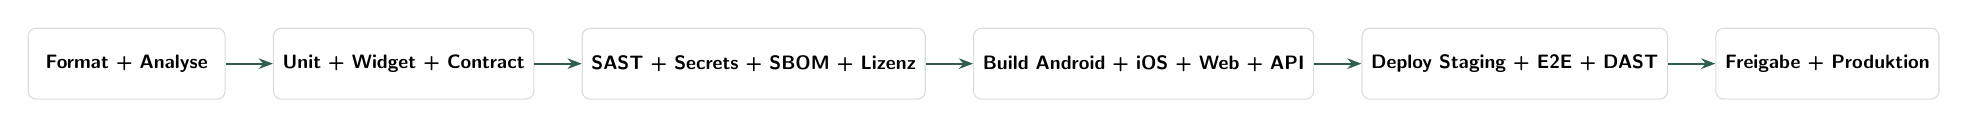
\begin{tikzpicture}[
  node distance=6mm,
  pipe/.style={draw=Line,fill=white,rounded corners=1mm,minimum width=25mm,minimum height=9mm,font=\scriptsize\bfseries,align=center},
  arr/.style={-{Stealth[length=1.8mm]},draw=Forest,line width=.65pt}]
  \node[pipe] (lint) {Format +\ Analyse};
  \node[pipe,right=of lint] (test) {Unit + Widget +\ Contract};
  \node[pipe,right=of test] (sec) {SAST + Secrets +\ SBOM + Lizenz};
  \node[pipe,right=of sec] (build) {Build Android +\ iOS + Web + API};
  \node[pipe,right=of build] (stage) {Deploy Staging +\ E2E + DAST};
  \node[pipe,right=of stage] (prod) {Freigabe +\ Produktion};
  \draw[arr] (lint)--(test); \draw[arr] (test)--(sec); \draw[arr] (sec)--(build);
  \draw[arr] (build)--(stage); \draw[arr] (stage)--(prod);
\end{tikzpicture}}
\end{center}

Signierte Releases entstehen ausschließlich aus geschützten Tags. Datenbankmigrationen laufen zuerst in Staging und besitzen Vorwärts- sowie Rückrollstrategie. Vor der Traffic-Umschaltung erfolgt ein Smoke-Test. iOS-Builds benötigen einen abgesicherten macOS-Runner; Signiermaterial liegt im Secret Management.

\subsection{Teststrategie}

\begin{tabularx}{\textwidth}{@{}p{32mm}X p{52mm}@{}}
\toprule
\textbf{Ebene} & \textbf{Zweck} & \textbf{Beispiele} \\
\midrule
Unit / Property & reine Domänenregeln schnell und vollständig & Scoring, Taxon-Synonyme, Levelabschluss, S-Kurven-/Quota-Berechnung \\
Widget / UI & Zustände, Semantik und Layout & Quizfeedback, Offlinebanner, große Schrift, Screenreaderlabels \\
Repository / Migration & lokale Speicherung und Versionswechsel & Isar/Web-Adapter, zwei Geräte, Abbruch, Datenbankupgrade \\
Contract & App-API und PlantNet-Adapter & OpenAPI, Fehlercodes, Quotenheader, Provider-Mocks \\
Integration & Komponenten mit PostgreSQL/Keycloak/Storage & Rollen, Upload, Worker, Löschlauf, Contentrelease \\
End-to-End & reale Kernreisen & Registrierung → Level → Quiz → Foto → Herbarium \\
Nichtfunktional & Last, Sicherheit, Restore, Accessibility & 100 RPS, 429-Ausfall, Pen-Test, Backup-Wiederherstellung \\
Fachreview & botanische und didaktische Richtigkeit & Stichprobe und Vollreview aller MVP-Inhalte \\
\bottomrule
\end{tabularx}

\subsection{Go-live-Checkliste}

\begin{multicols}{2}
\begin{itemize}
  \item alle MUSS-Anforderungen abgenommen;
  \item keine offenen kritischen/hohen Sicherheitsbefunde;
  \item 75 Arten und alle Quizfragen fachlich freigegeben;
  \item PlantNet-Vertrag/Quote und Attribution aktiv;
  \item Datenschutz, Minderjährigenfluss und Standortschutz freigegeben;
  \item Store-Metadaten und Account-Löschung geprüft;
  \item Lasttest auf 2x erwartete Spitzenstunde;
  \item Restore, Rollback und Incident-Übung bestanden;
  \item Monitoring, Alarmierung und Support besetzt;
  \item Staging-Smoke-Test und Produktionscheckliste grün;
  \item Open-Source-Repositories, Lizenzen und SBOM veröffentlicht;
  \item Kommunikations- und gestufter Rolloutplan freigegeben.
\end{itemize}
\end{multicols}

% -----------------------------------------------------------------------------
\section{Open-Source-Contribution und Governance}\label{sec:oss-governance}

\subsection{Lizenzvorschlag}

Als pragmatische Ausgangsbasis wird \textbf{Apache-2.0 für projektspezifischen Code} empfohlen: gut mit Strapi/Keycloak und institutioneller Nutzung vereinbar, patentfreundlich und App-Store-tauglich. Kuratierte Texte können -- bei geklärten Rechten -- unter \textbf{CC BY 4.0}, Medien je Asset unter CC BY/CC BY-SA oder abweichender klar dokumentierter Lizenz stehen. Marke, Logo und personenbezogene Forschungsdaten sind davon getrennt. Falls Netzwerk-Copyleft strategisch gewünscht ist, wird AGPL-3.0 für Serverteile separat rechtlich bewertet; eine unklare Mischlizenzierung ist zu vermeiden.

\subsection{Beitragsprozess}

\begin{enumerate}[leftmargin=7mm,label=\textcolor{Forest}{\arabic*.}]
  \item Öffentliche Roadmap und Issues mit Labels \Code{good first issue}, \Code{help wanted}, \Code{content}, \Code{security} und Anforderungs-ID.
  \item Fork/Branch, kleine fokussierte Commits, Tests und Dokumentation; DCO-Sign-off statt schwergewichtigem CLA, sofern die Rechtsprüfung zustimmt.
  \item Merge Request mit Motivation, betroffenen IDs, Screenshots bei UI, Migration, Datenschutz-/Accessibility-Auswirkung und Testnachweis.
  \item Mindestens ein technisches Review; bei Domänenänderungen zusätzlich botanisches/didaktisches Review. Maintainer führen Releases zusammen.
  \item Security-Befunde ausschließlich über private Disclosure-Adresse und SECURITY.md, nicht als öffentliches Issue.
  \item Inhalte werden über CMS-Export/Import und fachliche Quellen beigetragen; Bildrechte sind Pflichtbestandteil.
\end{enumerate}

\subsection{Governance}

Open Source bezeichnet bei Plantini nicht nur eine veröffentlichte Codeablage, sondern ein nachvollziehbares Betriebsmodell für gemeinsame Entwicklung. Ein Steering Committee aus Hochschule und Forschung, Produkt und Technik, Botanik und Didaktik sowie Betrieb schützt Mission und Gemeingut. Die tägliche Arbeit wird an benannte Maintainer delegiert. Architekturentscheidungen liegen als ADRs vor; größere Änderungen durchlaufen einen öffentlichen Request-for-Comments-Prozess (RFC). Sitzungsentscheidungen und Release Notes sind öffentlich, soweit Datenschutz und Sicherheit dies zulassen.

\subsubsection{Rollen, Mandate und Ernennung}

\begin{longtable}{@{}p{31mm}p{48mm}p{46mm}p{32mm}@{}}
\toprule
\textbf{Rolle} & \textbf{Mandat} & \textbf{Entscheidungsrecht} & \textbf{Bestellung / Kontrolle} \\
\midrule
\endhead
Steering Committee & Mission, Strategie, Finanzierung, Marke, Partnerschaften und Eskalation & Roadmap-Leitplanken, Budget, Governance-Änderungen, Maintainer-Berufung & ausgewogene institutionelle und fachliche Vertretung; feste Amtszeit; veröffentlichte Beschlüsse \\
Product Steward & bündelt Lernenden-, Lehrenden- und Betreiberbedarfe; pflegt priorisiertes Backlog & Priorisierung innerhalb freigegebener Roadmap; keine alleinige technische oder fachliche Freigabe & durch Steering Committee; regelmäßige Wirkungs- und Nutzungsberichte \\
Technical Maintainer & Architektur, Codequalität, API, Datenmigrationen, CI/CD und technische Reviews & Merge von Code nach Review; ADR-Vorschläge; kein Umgehen fachlicher Freigaben & nach nachweisbaren Beiträgen und Reviewqualität; Vier-Augen-Prinzip \\
Content Maintainer / Scientific Board & botanische Richtigkeit, Didaktik, Taxonomie, Quellen und Medienrechte & fachliche Freigabe von Steckbriefen, Quiz und Curricula; Sperre fehlerhafter Inhalte & Hochschulen, Botanik und Fachdidaktik; Interessenkonflikte offenlegen \\
Security Team & vertrauliche Meldungen, Triage, Koordination von Fix und Disclosure & zeitlich begrenztes Embargo und Notfallfreigabe; keine dauerhafte Geheim-Governance & kleinster notwendiger Personenkreis; dokumentierte Disclosure-Policy \\
Release Manager & Releasekalender, Versionierung, Signierung, Changelog, Artefakte und Rollback & Veröffentlichung einer technisch und fachlich freigegebenen Version & rotierende Maintainer-Rolle; Checkliste und reproduzierbare Pipeline \\
Contributor & Code, Tests, Übersetzungen, Dokumentation, UX oder Inhalte beitragen & Vorschlagsrecht über Issue, RFC und Merge Request; kein automatischer Merge-/Produktionszugriff & offen nach Code of Conduct, DCO und Beitragsleitfaden \\
Institutionelle Betreiber:in & eigene Instanz, IdP, lokale Rollen, Datenschutz und Support betreiben & lokale Konfiguration und Veröffentlichung im delegierten Mandat & Vertrag/Kooperation, Admin-Schulung und organisationsbezogene Rechte \\
Lernende / Lehrende / Tester:innen & Feedback, Barrieren, Inhaltsfehler und Forschungshinweise melden & Feedback- und Widerspruchsrecht; keine Pflicht zur öffentlichen Identität & App-Support, Pilotgruppen und öffentliche Community-Kanäle \\
\bottomrule
\end{longtable}

\subsubsection{Wie ein Beitrag bis in ein Release gelangt}

\begin{center}
\resizebox{.96\textwidth}{!}{%
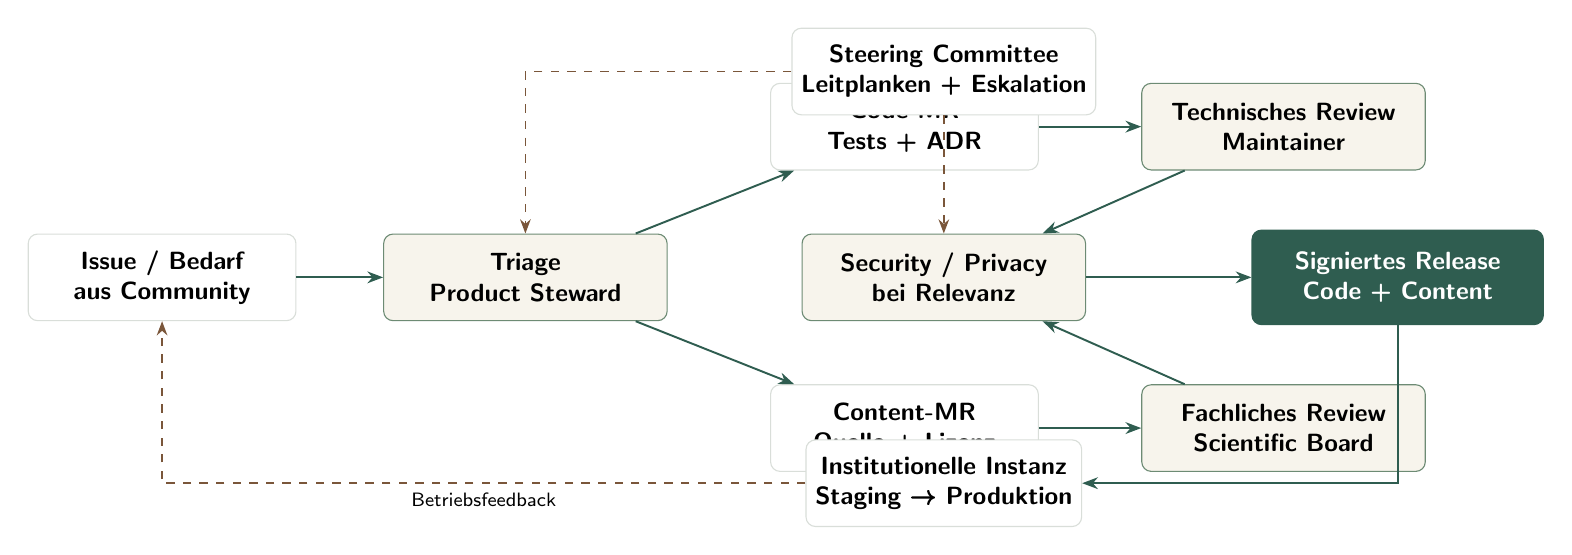
\begin{tikzpicture}[
  node distance=9mm and 11mm,
  role/.style={draw=Line,fill=white,rounded corners=1.2mm,minimum width=34mm,minimum height=11mm,align=center,font=\small\bfseries},
  gate/.style={draw=Sage,fill=Cream,rounded corners=1.2mm,minimum width=36mm,minimum height=11mm,align=center,font=\small\bfseries},
  release/.style={draw=Forest,fill=Forest,text=white,rounded corners=1.2mm,minimum width=37mm,minimum height=12mm,align=center,font=\small\bfseries},
  arr/.style={-{Stealth[length=2mm]},draw=Forest,line width=.7pt},
  policy/.style={-{Stealth[length=1.8mm]},draw=Bark,dashed,line width=.6pt}]
  \node[role] (need) {Issue / Bedarf\\aus Community};
  \node[gate,right=of need] (triage) {Triage\\Product Steward};
  \node[role,above right=8mm and 13mm of triage] (code) {Code-MR\\Tests + ADR};
  \node[role,below right=8mm and 13mm of triage] (content) {Content-MR\\Quelle + Lizenz};
  \node[gate,right=13mm of code] (techreview) {Technisches Review\\Maintainer};
  \node[gate,right=13mm of content] (scireview) {Fachliches Review\\Scientific Board};
  \node[gate,right=17mm of triage] (security) {Security / Privacy\\bei Relevanz};
  \node[release,right=21mm of security] (release) {Signiertes Release\\Code + Content};
  \node[role,above=15mm of security] (steering) {Steering Committee\\Leitplanken + Eskalation};
  \node[role,below=15mm of security] (operator) {Institutionelle Instanz\\Staging → Produktion};
  \draw[arr] (need) -- (triage);
  \draw[arr] (triage) -- (code);
  \draw[arr] (triage) -- (content);
  \draw[arr] (code) -- (techreview);
  \draw[arr] (content) -- (scireview);
  \draw[arr] (techreview) -- (security);
  \draw[arr] (scireview) -- (security);
  \draw[arr] (security) -- (release);
  \draw[arr] (release) |- (operator);
  \draw[policy] (steering) -- (security);
  \draw[policy] (steering.west) -| (triage.north);
  \draw[policy] (operator.west) -| node[pos=.25,below,font=\scriptsize]{Betriebsfeedback} (need.south);
\end{tikzpicture}}
\end{center}

Ein Beitrag kann rein technisch, rein inhaltlich oder kombiniert sein. Code und Content besitzen getrennte Prüfkriterien, treffen aber vor dem Release an einer gemeinsamen Sicherheits-, Datenschutz- und Integrationsschranke zusammen. Kritische Sicherheitskorrekturen dürfen zunächst vertraulich bearbeitet werden; nach dem koordinierten Release werden Ursache und Abhilfe angemessen offengelegt.

\begin{decisionbox}[title={\textbf{Wichtig: offen entwickeln, geschützt betreiben}}]
Öffentliche Repositories enthalten Quellcode, Infrastrukturvorlagen, anonymisierte Testdaten, offene Inhalte und Dokumentation. Produktionszugänge, personenbezogene Herbariumdaten, private Fotos, genaue Fundorte, Schlüssel, Backups und unveröffentlichte Sicherheitsmeldungen bleiben strikt geschützt. Contributor-, Maintainer-, CMS-Redaktions- und Produktionsrollen sind technisch getrennt. Eine Hochschule kann Plantini selbst hosten, ohne allen Community-Mitgliedern Zugriff auf ihre Instanz zu geben.
\end{decisionbox}

\subsubsection{Vorteile des Modells}

\begin{tabularx}{\textwidth}{@{}p{35mm}X X@{}}
\toprule
\textbf{Vorteil} & \textbf{Wirkmechanismus bei Plantini} & \textbf{Konkreter Nutzen} \\
\midrule
Nachhaltigkeit & mehrere Institutionen können Maintainer stellen; dokumentierte Übergabe und reproduzierbarer Betrieb & Fortführung bei Personalwechsel oder auslaufender Einzelförderung \\
Wissenschaftliche Transparenz & Versionen von Code, Lernlogik, Fragekatalog und Auswertungsdefinitionen sind referenzierbar & Studien werden nachvollziehbarer und Ergebnisse besser reproduzierbar \\
Schnellere Regionalisierung & lokale Hochschulen ergänzen Sprachen, Ökosysteme und Arten über definierte Contentpakete & internationale Expansion ohne zentralen Entwicklungsengpass \\
Höhere Fachqualität & getrenntes technisches, botanisches, didaktisches und rechtliches Review & weniger fehlerhafte Artenzuordnungen, Fragen und Medienlizenzen \\
Digitale Souveränität & offene Formate, Self-Hosting, dokumentierter Export und austauschbare Adapter & keine Abhängigkeit von einem einzelnen Betreiber oder Cloudanbieter \\
Lehre und Transfer & Studierende können abgegrenzte Issues, Übersetzungen, Tests und Module beitragen & reale Projektarbeit, Nachwuchsgewinnung und Wissenstransfer \\
Sicherheit & öffentliche Prüfbarkeit plus vertraulicher Disclosure-Weg und signierte Releases & Fehler können organisationsübergreifend gefunden und koordiniert behoben werden \\
Förderfähigkeit und Skalierung & Ergebnisse bleiben als öffentliches Gemeingut nutzbar; Partnerleistungen werden sichtbar & Investitionen wirken über ein einzelnes Pilotprojekt hinaus \\
\bottomrule
\end{tabularx}

Die Vorteile entstehen nicht automatisch durch Veröffentlichung. Erforderlich sind finanzierte Maintainer-Zeit, verlässliche Reviews, ein aktiver Code of Conduct, eine klare Markenregelung, planbare Releases und ein Budget für Infrastruktur, Security und fachliche Qualität. Diese Betriebsaufgaben sind daher Teil der Finanzierung und nicht unentgeltlich auf die Community zu verlagern (\R{NFA032}).

% -----------------------------------------------------------------------------
\section{Ausweitung auf weitere Regionen und Sprachen}

\begin{tabularx}{\textwidth}{@{}p{36mm}X X@{}}
\toprule
\textbf{Dimension} & \textbf{Bereits im MVP vorzusehen} & \textbf{Vor regionalem Rollout zu klären} \\
\midrule
Sprache & Locale-IDs, Fallback, plural-/längenfeste UI vermeiden & professionelle Übersetzung, botanische Trivialnamen, leichte Sprache \\
Ökosysteme & Region/Flora nicht fest im Code, Contentpakete & lokale Definitionen, Saisonalität, Lehrplan, Expert:innenreview \\
Taxonomie & interne Taxon-ID, Synonyme, externe Referenzen & lokale Artenlisten, invasive/geschützte Arten, taxonomische Quelle \\
PlantNet & konfigurierbares Projekt/Referenzial und Sprache & Abdeckung, Vertrag, Modellgüte, Quote und Attribution in Region \\
Recht & konfigurierbare Einwilligungs-/Hinweistexte & Datenschutz, Minderjährigenalter, Karten-/Standortrecht, Store-Regeln \\
Artenschutz & private/vergröberte Geodaten & Schutz sensibler Arten, Betretungs- und Sammelverbote \\
Forschung & versionierter Eventkatalog, Opt-in & lokales Ethikvotum, Datentransfer, Übersetzung der Einwilligung \\
Betrieb & portable Container/IaC, EU-Region & Latenz, Datenresidenz, Supportzeiten, lokale Partner \\
\bottomrule
\end{tabularx}

Empfohlen ist eine Expansion in Stufen: (1) Österreich/Schweiz mit rechtlicher und inhaltlicher Anpassung, (2) weitere europäische biogeografische Regionen, (3) außereuropäische Pilotregion mit lokaler Hochschule und Botanikpartner. Jeder Rollout beginnt mit Content-/Rechts-Gap-Analyse und einem kleinen Feldpilot.

% -----------------------------------------------------------------------------
\section{Finanzierung und Fördermöglichkeiten}\label{sec:funding}

\subsection{Geschätzter Entwicklungsbedarf}

Die folgende Kostenspanne ist eine Vollkosten-/Vergabeplanung einschließlich Arbeitgeberkosten bzw. externer Tagessätze, nicht nur Entwicklerlohn. Sie basiert auf 75 kumulativen Arten und dem vollständigen MVP. Beträge verstehen sich netto und müssen nach Beschaffungs-/Förderrecht konkretisiert werden.

\begin{longtable}{@{}p{56mm}p{27mm}p{27mm}p{47mm}@{}}
\toprule
\textbf{Arbeitspaket} & \textbf{Untergrenze} & \textbf{Obergrenze} & \textbf{Annahme} \\
\midrule
\endhead
Projektleitung, Product, Forschung & 60.000 € & 85.000 € & ca. 0,7 FTE über 9 Monate \\
UX, Designsystem, Accessibility & 30.000 € & 50.000 € & ca. 0,4 FTE + Tests \\
Flutter-App & 180.000 € & 250.000 € & zwei Entwickler:innen über 8--9 Monate \\
Backend, SSO, DevOps, Betriebsvorbereitung & 90.000 € & 135.000 € & ca. 1 FTE + Security/Infra \\
QA, Testautomation, Penetrationstest, Stores & 45.000 € & 75.000 € & QA-Kapazität + externe Prüfung \\
CMS-Konfiguration und Content-Pipeline & 35.000 € & 60.000 € & Builder, Import, Reviewworkflow \\
Botanische Inhalte, Bilder, Review (75 Arten) & 70.000 € & 125.000 € & 750--1.350 Fachstunden + Rechte \\
Leveldidaktik, Quiz und Feldpilot & 40.000 € & 70.000 € & Lernziele, Fragen, Evaluation \\
Recht, Datenschutz, Infrastruktur, Kontingente & 25.000 € & 50.000 € & DSFA/Verträge, Hosting, Geräte, Gebühren \\
\midrule
Zwischensumme & 575.000 € & 900.000 € & vor Reserve \\
Risikoreserve 10--15\,\% & 60.000 € & 120.000 € & Scope, Store, Content, SSO, Provider \\
\midrule
\textbf{Empfohlener Finanzierungsrahmen} & \textbf{635.000 €} & \textbf{1.020.000 €} & Produktionsreifer MVP bis April 2027 \\
\bottomrule
\end{longtable}

Ein sehr schlanker Prototyp ist mit internen Vorleistungen günstiger möglich, würde aber typischerweise Abstriche bei Inhalten, Plattformbreite, Security, Forschung oder Betriebsreife machen. Bei 225 statt 75 Arten sind zusätzlich grob 140.000--260.000 € für Inhalte, Medien, Quiz, Review und Tests einzuplanen.

\subsection{Betrieb ab Go-live}

Für das erste volle Betriebsjahr werden \textbf{140.000--280.000 €} empfohlen:

\begin{itemize}
  \item 0,8--1,5 FTE Wartung, Support, Releases und Sicherheit: 85.000--170.000 €;
  \item Hosting, Backups, Monitoring, Storage/CDN und Geräte: 20.000--45.000 €;
  \item PlantNet: 0 € im genehmigten Non-Profit-Modell bis zu etwa 35.000 € Reserve bei kommerziellem/hohem Volumen;
  \item laufende Fachredaktion, neue Inhalte und Übersetzungen: 25.000--50.000 €.
\end{itemize}

\subsection{Passende Förderwege (Stand 17.07.2026)}

\begin{longtable}{@{}p{36mm}p{28mm}p{52mm}p{40mm}@{}}
\toprule
\textbf{Instrument} & \textbf{Potenzieller Beitrag} & \textbf{Fit und Bedingungen} & \textbf{Zeitkritik} \\
\midrule
\endhead
Universität / Fakultäten / QSM / Transfer & 150.000--300.000 € plus Stellen/Sachmittel & Kernfinanzierung für Lehre, Forschungsinfrastruktur, Personal, Geräte und Vorlauf; interne Verfahren und Zweckbindung prüfen. & als Brücke sofort nötig \\
Land Baden-Württemberg / MWK-Linien & 100.000--400.000 € je Ausschreibung & digitale Lehre, Transfer, MINT/BNE und Hochschulkooperation; konkrete offene Linie mit Forschungsförderung prüfen. & Bescheid darf nicht kritischer Pfad sein \\
Vector Stiftung „MINT-Innovationen“ & bis 100.000 € / max. 2 Jahre & Forschende aller Karrierestufen in BW; risikoreiche MINT-Idee, nächster Call laut Seite Herbst 2026.\Src{12} & gut für Forschungs-/Adaptivitätsmodul \\
Deutsche Bundesstiftung Umwelt & projektspezifisch, bei Hochschulen bis zu 100\,\% der Ausgaben & innovativ, modellhaft, praxisnah, konkrete Umweltentlastung; Skizzen jederzeit, aber keine bereits begonnenen Vorhaben.\Src{13} & eigener noch nicht begonnener WP/Pilot \\
Stiftung Innovation in der Hochschullehre „Freiraum“ & abhängig vom Call & innovative Lernprozesse; nächste Ausschreibung laut Stiftung Anfang 2027.\Src{14} & eher Evaluation/Skalierung nach Go-live \\
BMFTR / Citizen Science & callabhängig & hoher Fit bei echter Beteiligung von Bürger:innen an relevanter Forschung; frühere Richtlinien fordern wissenschaftliche Standards und Datenkonzept.\Src{15} & aktuellen Call beobachten \\
EU / Horizon Europe / Erasmus+ / Interreg & typ. 150.000 € bis mehrjähriger Verbund & Internationalisierung, Biodiversität, Wissenschaftskommunikation, Hochschul-/Schulpartnerschaften; hoher Antrag-/Koordinationsaufwand.\Src{16} & für Phase 2 ab 2027 \\
PlantNet Non-Profit-Kontingent & Sachleistung / variable Kostenersparnis & Bildung/Wissenschaft, auf Anfrage mehr als 500 Identifikationen/Tag bzw. Burst; Attribution erforderlich.\Src{11} & vor Feldpilot vertraglich klären \\
\bottomrule
\end{longtable}

\subsection{Empfohlener Finanzierungsmix}

\begin{decisionbox}[title={\textbf{Finanzierungsstrategie für den April-Go-live}}]
\begin{enumerate}[leftmargin=7mm,label=\textcolor{Forest}{\arabic*.}]
  \item \textbf{Sofortige Kern-/Brückenfinanzierung 300.000--450.000 €} durch Universität, Land/Projektpartner und verbindliche Eigenleistungen für Architektur, App, Backend und erste Inhalte.
  \item \textbf{Externe Pakete 200.000--400.000 €} sauber getrennt beantragen: DBU für modellhaften Biodiversitäts-/Bildungspilot, Vector für risikoreiche Lern-/Forschungsinnovation, ggf. private Stiftungen.
  \item \textbf{In-kind 80.000--150.000 €} durch botanische Institute, Hochschulen und Schulen: Fachreview, Bildbestände, Pilotflächen, wissenschaftliche Mitarbeit, Geräte und Kommunikation.
  \item \textbf{Betriebszusage ab 2027 mindestens 140.000 €/Jahr} vor Go-live sichern; ein befristet gefördertes Produkt ohne Wartungs-, Security- und Inhaltsbudget ist nicht nachhaltig.
\end{enumerate}
\end{decisionbox}

Kosten dürfen nicht doppelt gefördert werden. Für DBU und ähnliche Programme ist „noch nicht begonnen“ entscheidend; bereits gestartete Entwicklung ist ggf. als Eigenvorleistung abzugrenzen und ein eigenständiges, noch nicht begonnenes Forschungs-/Transferarbeitspaket zu beantragen. Die Förderfähigkeit muss jeweils schriftlich mit Förderberatung und Drittmittelverwaltung geklärt werden.

% -----------------------------------------------------------------------------
\section{Risiken, Annahmen und Entscheidungen}

\begin{longtable}{@{}p{13mm}p{41mm}p{20mm}p{83mm}@{}}
\toprule
\textbf{ID} & \textbf{Risiko} & \textbf{Bewertung} & \textbf{Gegenmaßnahme / Entscheidungspunkt} \\
\midrule
\endhead
R-01 & 25/50/75 je Level vs. je Ökosystem unklar & hoch & A-01 bis 31.07.2026 freigeben; Budget/Plan automatisch anpassen. \\
R-02 & Isar-Webpfad nicht produktionsreif & hoch & Spike bis 28.08.2026; Persistenzport und IndexedDB/Drift-WASM-Fallback. \\
R-03 & PlantNet-Quote/Burst reicht nicht & hoch & Non-Profit-Vertrag oder Budget vor Pilot; Queue, Warnung, harte Tagesreserve. \\
R-04 & Förderbescheid kommt nach Entwicklungsstart & hoch & Kernfinanzierung unabhängig sichern; beantragte Arbeitspakete klar noch nicht beginnen. \\
R-05 & Google/Apple/Uni-SSO und Account-Linking verzögern Stores & mittel/hoch & Keycloak-Spike früh; Test-IdP; Provider-Checklisten und manuelle Admin-Einladung. \\
R-06 & Minderjährigen-, Foto- und GPS-Verarbeitung & hoch & DSFA-Screening, Privacy UX, private/vergröberte Orte, getrennte Forschungseinwilligung. \\
R-07 & Bildrechte oder fachliches Review fehlen & hoch & Rechte als Pflichtfeld; Content-Kanban, frühe Gap-Liste, keine ungeprüfte Veröffentlichung. \\
R-08 & iOS-Signierung/Store-Review verpasst Termin & mittel & Mac-Runner und Storekonten bis Oktober; TestFlight ab Januar; Einreichung Ende März. \\
R-09 & Kampagne erzeugt stärkere Burstlast als Modell & mittel & 2x Lasttest, Rate Limits, CDN, gestufter Rollout, horizontale Worker. \\
R-10 & Open-Source-Projekt verliert Maintainer & mittel & Steering Committee, dokumentierte Rollen, finanzierter Betrieb, Releasekalender, Contributor-Onboarding. \\
R-11 & Taxonomische Änderungen brechen Fortschritt & mittel & interne Taxon-ID, Synonyme/Versionierung, Migration und Fachreview. \\
R-12 & 75 Arten bis Februar nicht vollständig & hoch & Inhaltsgruppen ab Juli parallel; Priorisierung und wöchentliches Burndown; keine Softwareabhängigkeit. \\
\bottomrule
\end{longtable}

% -----------------------------------------------------------------------------
\section{Traceability und Abnahmematrix}\label{sec:traceability}

\begin{longtable}{@{}p{35mm}p{60mm}p{63mm}@{}}
\toprule
\textbf{Projektziel} & \textbf{Zentrale Anforderungen} & \textbf{Abnahmenachweis} \\
\midrule
\endhead
Spielerische Pflanzenkunde & \R{FA020}--\R{FA029}, \R{NFA017}, \R{NFA028} & E2E-Lernreise, Fachdidaktikreview, Usabilitytest \\
Dynamische Inhalte & \R{FA010}--\R{FA017}, \R{FA050}--\R{FA054} & viertes Level ohne App-Release veröffentlichen \\
Naturtransfer / PlantNet & \R{FA030}--\R{FA040}, \R{NFA030} & Feldpilot, Provider-Mock/Quote, Unsicherheitsfälle \\
Persönliches Herbarium & \R{FA036}--\R{FA039}, \R{NFA014} & Offline-Fund, Sync über zwei Geräte, Export/Löschung \\
Offline-Fähigkeit & \R{FA041}--\R{FA045}, \R{NFA020} & Flugmodus-E2E, Abbruch-/Migrations- und Konflikttests \\
Institutionelle Plattform & \R{FA003}, \R{FA006}, \R{FA061}, \R{NFA015} & Test-IdP, Rechte-Matrix, Organisationsisolation \\
Open Source / Nachhaltigkeit & \R{NFA001}, \R{NFA026}, \R{NFA027}, \R{NFA032} & Lizenzscan, frischer Restore/Build, öffentliche Dokumentation, exemplarischer Code-/Content-Beitrag und Governance-Entscheid \\
Forschung mit Datenschutz & \R{FA070}--\R{FA074}, \R{NFA012}, \R{NFA013} & Einwilligungs-/Widerruftest, Eventkatalog, genehmigter Export \\
Skalierbarer Betrieb & \R{NFA005}--\R{NFA008}, \R{NFA024} & Lasttest, SLO-Dashboard, Restore-/Incident-Übung \\
Barrierefreier Zugang & \R{NFA016}, \R{NFA018}, \R{NFA019} & WCAG-Test, Screenreader/Tastatur, Plattformmatrix \\
\bottomrule
\end{longtable}

\subsection{Erfolgskriterien nach Go-live}

Produktmetriken werden erst nach Baseline/Pilot mit Zielwerten versehen. Empfohlen sind: Aktivierung (erstes Lernmodul), Levelabschluss, Wiederkehr nach 7/30 Tagen, Wissenszuwachs in freiwilligen Pre-/Post-Tests, Anteil erfolgreich synchronisierter Offlineereignisse, Identifikationsquote und -unsicherheit, Crash-free sessions, Accessibility-Befunde, Supportzeit und Inhaltfehlerquote. Reine Nutzungsdauer ist kein Bildungsziel.

% -----------------------------------------------------------------------------
\section{Quellen und Entscheidungsgrundlagen}

\small
\begin{enumerate}[leftmargin=9mm,label={\textcolor{Forest}{[\arabic*]}}]
  \hypertarget{src:1}{}\item A. Zeqiri, T. Wagner, J. Grüneberg, E. Rukzio: \emph{BotaXplore: Enhancing Visitor Engagement and Learning in Botanical Gardens Through Mobile Technology}, CHI EA 2026, Universität Ulm. \href{https://www.uni-ulm.de/fileadmin/website_uni_ulm/iui.inst.100/institut/mitarbeiterbereiche/zeqiri/papers/preprint_botaxplore.pdf}{Preprint / DOI 10.1145/3772363.3799272}.
  \hypertarget{src:2}{}\item Pl@ntNet: \href{https://my.plantnet.org/doc/api/identify}{Single-species identification API}; Bilder, Organangaben, Scores, Ausgabeformat und Route.
  \hypertarget{src:3}{}\item Pl@ntNet: \href{https://my.plantnet.org/doc/api/quota}{Quota management}; tägliche Kontingente, RateLimit-Header und Quotenendpunkte.
  \hypertarget{src:4}{}\item Strapi: \href{https://github.com/strapi/strapi}{offizielles Repository}; Content-Type-Builder, REST/GraphQL, Rollen, Media Library, i18n, Draft/Publish und PostgreSQL.
  \hypertarget{src:5}{}\item Strapi: \href{https://strapi.io/pricing-cms}{CMS Pricing / Open-Source Edition}; MIT-Lizenz und unbegrenzte Self-hosted-Nutzung laut Anbieter.
  \hypertarget{src:6}{}\item Payload: \href{https://payloadcms.com/docs/getting-started/what-is-payload}{What is Payload?}; Admin Panel, Datenbank, REST/GraphQL, Auth, Access Control und Uploads.
  \hypertarget{src:7}{}\item Directus: \href{https://directus.io/pricing}{Pricing und Lizenz-/Tierhinweise}; Organisationsgrenzen und SSO-Verfügbarkeit.
  \hypertarget{src:8}{}\item Supabase: \href{https://supabase.com/docs/guides/getting-started/architecture}{Architecture}; PostgreSQL, Auth, APIs, Storage und Open-Source-Komponenten.
  \hypertarget{src:9}{}\item Keycloak: \href{https://www.keycloak.org/}{Projekt- und Funktionsübersicht}; OIDC, OAuth 2.0, SAML, Social Login, Identity Brokering, MFA und Administration.
  \hypertarget{src:10}{}\item Isar: \href{https://github.com/isar/isar/issues/1689}{Maintainer-/Community-Statusdiskussion} und \href{https://github.com/isar/isar/discussions/1143}{Web-Supportdiskussion}; Grundlage für den verpflichtenden Web-Spike.
  \hypertarget{src:11}{}\item Pl@ntNet: \href{https://my.plantnet.org/pricing}{Pricing and conditions}; Free-, Pro- und Non-Profit-Angebot, Stand Abruf 17.07.2026.
  \hypertarget{src:12}{}\item Vector Stiftung: \href{https://vector-stiftung.de/ausschreibungen/mint-innovationen/}{MINT-Innovationen}; nächster Call Herbst 2026, bis 100.000 € für maximal zwei Jahre.
  \hypertarget{src:13}{}\item Deutsche Bundesstiftung Umwelt (DBU): \href{https://www.dbu.de/foerderung/projektfoerderung/}{Projektförderung}. Skizzen sind jederzeit möglich; begonnene Vorhaben sind ausgeschlossen. Hochschulen können bis zu 100\,\% der Projektausgaben erhalten.
  \hypertarget{src:14}{}\item Stiftung Innovation in der Hochschullehre: \href{https://stiftung-hochschullehre.de/foerderung/freiraum/}{Freiraum}; nächste Ausschreibung laut Website Anfang 2027.
  \hypertarget{src:15}{}\item Bundesministerium für Forschung: \href{https://www.bmbf.de/DE/Forschung/Gesellschaft/Beteiligungdergesellschaft/CitizenScience/citizenscience.html}{Citizen Science} sowie frühere Förderrichtlinien als strategischer Fit; aktuelle Ausschreibung jeweils prüfen.
  \hypertarget{src:16}{}\item Europäische Kommission: \href{https://commission.europa.eu/funding-tenders/find-funding/eu-funding-programmes_en}{EU funding programmes}; Horizon Europe und weitere Programme 2021--2027.
  \hypertarget{src:17}{}\item Europäische Kommission: \href{https://commission.europa.eu/law/law-topic/data-protection_en}{Data protection in the EU}; DSGVO-Grundsätze und internationale Datenübermittlung.
\hypertarget{src:18}{}\item W3C: \href{https://www.w3.org/TR/WCAG22/}{Web Content Accessibility Guidelines (WCAG) 2.2}.
\end{enumerate}
\normalsize

\begin{riskbox}[title={\textbf{Hinweis zu Recht und Förderung}}]
Dieses Dokument ist eine technische und organisatorische Planung, keine Rechts- oder Förderberatung. Datenschutz, Minderjährigeneinwilligung, Bild-/Kartennutzung, App-Store-Regeln, PlantNet-Vertrag und Förderfähigkeit sind vor Bindung von Mitteln durch die zuständigen Stellen verbindlich zu prüfen. Programmstatus und Konditionen können sich nach dem 17. Juli 2026 ändern.
\end{riskbox}

\vfill
\begin{center}
\textcolor{Sage}{\rule{35mm}{0.6pt}}\\[2mm]
 {\small\textcolor{Muted}{Ende des Anforderungsdokuments · Version 1.2}}
\end{center}

\end{document}
